% **************************************************************************************************************
% A Classic Thesis Style
% An Homage to The Elements of Typographic Style
%
% Copyright (C) 2018 André Miede and Ivo Pletikosić
%
% If you like the style then I would appreciate a postcard. My address
% can be found in the file ClassicThesis.pdf. A collection of the
% postcards I received so far is available online at
% http://postcards.miede.de
%
% License:
% This program is free software; you can redistribute it and/or modify
% it under the terms of the GNU General Public License as published by
% the Free Software Foundation; either version 2 of the License, or
% (at your option) any later version.
%
% This program is distributed in the hope that it will be useful,
% but WITHOUT ANY WARRANTY; without even the implied warranty of
% MERCHANTABILITY or FITNESS FOR A PARTICULAR PURPOSE.  See the
% GNU General Public License for more details.
%
% You should have received a copy of the GNU General Public License
% along with this program; see the file COPYING.  If not, write to
% the Free Software Foundation, Inc., 59 Temple Place - Suite 330,
% Boston, MA 02111-1307, USA.
%
% PLEASE SEE ALSO THE AUTHORS' NOTE REGARDING THIS LICENSE
% IN THE DOCUMENTATION (ClassicThesis.pdf --> Chapter 1 / Chapter01.tex)
% **************************************************************************************************************
\RequirePackage{silence} % :-\
    \WarningFilter{scrreprt}{Usage of package `titlesec'}
    %\WarningFilter{scrreprt}{Activating an ugly workaround}
    \WarningFilter{titlesec}{Non standard sectioning command detected}
\documentclass[ twoside,openright,titlepage,numbers=noenddot,%1headlines,
                headinclude,footinclude,cleardoublepage=empty,abstract=on,
                BCOR=5mm,paper=a4,fontsize=11pt
                ]{scrreprt}

%********************************************************************
% Note: Make all your adjustments in here
%*******************************************************
% ****************************************************************************************************
% classicthesis-config.tex
% formerly known as loadpackages.sty, classicthesis-ldpkg.sty, and classicthesis-preamble.sty
% Use it at the beginning of your ClassicThesis.tex, or as a LaTeX Preamble
% in your ClassicThesis.{tex,lyx} with % ****************************************************************************************************
% classicthesis-config.tex
% formerly known as loadpackages.sty, classicthesis-ldpkg.sty, and classicthesis-preamble.sty
% Use it at the beginning of your ClassicThesis.tex, or as a LaTeX Preamble
% in your ClassicThesis.{tex,lyx} with % ****************************************************************************************************
% classicthesis-config.tex
% formerly known as loadpackages.sty, classicthesis-ldpkg.sty, and classicthesis-preamble.sty
% Use it at the beginning of your ClassicThesis.tex, or as a LaTeX Preamble
% in your ClassicThesis.{tex,lyx} with \input{classicthesis-config}
% ****************************************************************************************************
% If you like the classicthesis, then I would appreciate a postcard.
% My address can be found in the file ClassicThesis.pdf. A collection
% of the postcards I received so far is available online at
% http://postcards.miede.de
% ****************************************************************************************************


% ****************************************************************************************************
% 0. Set the encoding of your files. UTF-8 is the only sensible encoding nowadays. If you can't read
% äöüßáéçèê∂åëæƒÏ€ then change the encoding setting in your editor, not the line below. If your editor
% does not support utf8 use another editor!
% ****************************************************************************************************
\PassOptionsToPackage{utf8}{inputenc}
  \usepackage{inputenc}

\PassOptionsToPackage{T1}{fontenc} % T2A for cyrillics
  \usepackage{fontenc}


% ****************************************************************************************************
% 1. Configure classicthesis for your needs here, e.g., remove "drafting" below
% in order to deactivate the time-stamp on the pages
% (see ClassicThesis.pdf for more information):
% ****************************************************************************************************
\PassOptionsToPackage{drafting=true,    % print version information on the bottom of the pages
  tocaligned=false, % the left column of the toc will be aligned (no indentation)
  dottedtoc=false,  % page numbers in ToC flushed right
  eulerchapternumbers=true, % use AMS Euler for chapter font (otherwise Palatino)
  linedheaders=false,       % chaper headers will have line above and beneath
  floatperchapter=true,     % numbering per chapter for all floats (i.e., Figure 1.1)
  eulermath=true,  % use awesome Euler fonts for mathematical formulae (only with pdfLaTeX)
  beramono=true,    % toggle a nice monospaced font (w/ bold)
  palatino=true,    % deactivate standard font for loading another one, see the last section at the end of this file for suggestions
  style=arsclassica % classicthesis, arsclassica
}{classicthesis}


% ****************************************************************************************************
% 2. Personal data and user ad-hoc commands (insert your own data here)
% ****************************************************************************************************
\newcommand{\myTitle}{Statistical Learning Approaches for the Control of Stormwater Systems\xspace}
\newcommand{\mySubtitle}{\xspace}
\newcommand{\myDegree}{Doctor of Philosophy\xspace}
\newcommand{\myName}{Abhiram Mullapudi\xspace}
\newcommand{\myProf}{Put name here\xspace}
\newcommand{\myOtherProf}{Put name here\xspace}
\newcommand{\mySupervisor}{Put name here\xspace}
\newcommand{\myFaculty}{Put data here\xspace}
\newcommand{\myDepartment}{Department of Civil and Environmental Engineering\xspace}
\newcommand{\myUni}{University of Michigan\xspace}
\newcommand{\myLocation}{Ann Arbor\xspace}
\newcommand{\myTime}{June 2020\xspace}
\newcommand{\myVersion}{0.1}

% ********************************************************************
% Setup, finetuning, and useful commands
% ********************************************************************
\providecommand{\mLyX}{L\kern-.1667em\lower.25em\hbox{Y}\kern-.125emX\@}
\newcommand{\ie}{i.\,e.}
\newcommand{\Ie}{I.\,e.}
\newcommand{\eg}{e.\,g.}
\newcommand{\Eg}{E.\,g.}
% ****************************************************************************************************


% ****************************************************************************************************
% 3. Loading some handy packages
% ****************************************************************************************************
% ********************************************************************
% Packages with options that might require adjustments
% ********************************************************************
\PassOptionsToPackage{american}{babel} % change this to your language(s), main language last
% Spanish languages need extra options in order to work with this template
%\PassOptionsToPackage{spanish,es-lcroman}{babel}
    \usepackage{babel}

\usepackage{csquotes}
\PassOptionsToPackage{%
  %backend=biber,bibencoding=utf8, %instead of bibtex
  backend=bibtex8,bibencoding=ascii,%
  language=auto,%
  style=numeric-comp,%
  %style=authoryear-comp, % Author 1999, 2010
  %bibstyle=authoryear,dashed=false, % dashed: substitute rep. author with ---
  sorting=nyt, % name, year, title
  maxbibnames=5, % default: 3, et al.
  %backref=true,%
  natbib=true % natbib compatibility mode (\citep and \citet still work)
}{biblatex}
    \usepackage{biblatex}

\PassOptionsToPackage{fleqn}{amsmath}       % math environments and more by the AMS
  \usepackage{amsmath}

% ********************************************************************
% General useful packages
% ********************************************************************
\usepackage{graphicx} %
\usepackage{scrhack} % fix warnings when using KOMA with listings package
\usepackage{xspace} % to get the spacing after macros right
\PassOptionsToPackage{printonlyused,smaller}{acronym}
  \usepackage{acronym} % nice macros for handling all acronyms in the thesis
  %\renewcommand{\bflabel}[1]{{#1}\hfill} % fix the list of acronyms --> no longer working
  %\renewcommand*{\acsfont}[1]{\textsc{#1}}
  %\renewcommand*{\aclabelfont}[1]{\acsfont{#1}}
  %\def\bflabel#1{{#1\hfill}}
  \def\bflabel#1{{\acsfont{#1}\hfill}}
  \def\aclabelfont#1{\acsfont{#1}}
% ****************************************************************************************************
%\usepackage{pgfplots} % External TikZ/PGF support (thanks to Andreas Nautsch)
%\usetikzlibrary{external}
%\tikzexternalize[mode=list and make, prefix=ext-tikz/]
% ****************************************************************************************************


% ****************************************************************************************************
% 4. Setup floats: tables, (sub)figures, and captions
% ****************************************************************************************************
\usepackage{tabularx} % better tables
  \setlength{\extrarowheight}{3pt} % increase table row height
\newcommand{\tableheadline}[1]{\multicolumn{1}{l}{\spacedlowsmallcaps{#1}}}
\newcommand{\myfloatalign}{\centering} % to be used with each float for alignment
\usepackage{subfig}
% ****************************************************************************************************


% ****************************************************************************************************
% 5. Setup code listings
% ****************************************************************************************************
\usepackage{listings}
%\lstset{emph={trueIndex,root},emphstyle=\color{BlueViolet}}%\underbar} % for special keywords
\lstset{language=[LaTeX]Tex,%C++,
  morekeywords={PassOptionsToPackage,selectlanguage},
  keywordstyle=\color{RoyalBlue},%\bfseries,
  basicstyle=\small\ttfamily,
  %identifierstyle=\color{NavyBlue},
  commentstyle=\color{Green}\ttfamily,
  stringstyle=\rmfamily,
  numbers=none,%left,%
  numberstyle=\scriptsize,%\tiny
  stepnumber=5,
  numbersep=8pt,
  showstringspaces=false,
  breaklines=true,
  %frameround=ftff,
  %frame=single,
  belowcaptionskip=.75\baselineskip}
  %frame=L

% ****************************************************************************************************




% ****************************************************************************************************
% 6. Last calls before the bar closes
% ****************************************************************************************************
% ********************************************************************
% Her Majesty herself
% ********************************************************************
\usepackage{classicthesis}


% ********************************************************************
% Fine-tune hyperreferences (hyperref should be called last)
% ********************************************************************
\hypersetup{%
  %draft, % hyperref's draft mode, for printing see below
  colorlinks=true, linktocpage=true, pdfstartpage=3, pdfstartview=FitV,%
  % uncomment the following line if you want to have black links (e.g., for printing)
  %colorlinks=false, linktocpage=false, pdfstartpage=3, pdfstartview=FitV, pdfborder={0 0 0},%
  breaklinks=true, pageanchor=true,%
  pdfpagemode=UseNone, %
  % pdfpagemode=UseOutlines,%
  plainpages=false, bookmarksnumbered, bookmarksopen=true, bookmarksopenlevel=1,%
  hypertexnames=true, pdfhighlight=/O,%nesting=true,%frenchlinks,%
  urlcolor=CTurl, linkcolor=CTlink, citecolor=CTcitation, %pagecolor=RoyalBlue,%
  %urlcolor=Black, linkcolor=Black, citecolor=Black, %pagecolor=Black,%
  pdftitle={\myTitle},%
  pdfauthor={\textcopyright\ \myName, \myUni, \myFaculty},%
  pdfsubject={},%
  pdfkeywords={},%
  pdfcreator={pdfLaTeX},%
  pdfproducer={LaTeX with hyperref and classicthesis}%
}


% ********************************************************************
% Setup autoreferences (hyperref and babel)
% ********************************************************************
% There are some issues regarding autorefnames
% http://www.tex.ac.uk/cgi-bin/texfaq2html?label=latexwords
% you have to redefine the macros for the
% language you use, e.g., american, ngerman
% (as chosen when loading babel/AtBeginDocument)
% ********************************************************************
\makeatletter
\@ifpackageloaded{babel}%
  {%
    \addto\extrasamerican{%
      \renewcommand*{\figureautorefname}{Figure}%
      \renewcommand*{\tableautorefname}{Table}%
      \renewcommand*{\partautorefname}{Part}%
      \renewcommand*{\chapterautorefname}{Chapter}%
      \renewcommand*{\sectionautorefname}{Section}%
      \renewcommand*{\subsectionautorefname}{Section}%
      \renewcommand*{\subsubsectionautorefname}{Section}%
    }%
    \addto\extrasngerman{%
      \renewcommand*{\paragraphautorefname}{Absatz}%
      \renewcommand*{\subparagraphautorefname}{Unterabsatz}%
      \renewcommand*{\footnoteautorefname}{Fu\"snote}%
      \renewcommand*{\FancyVerbLineautorefname}{Zeile}%
      \renewcommand*{\theoremautorefname}{Theorem}%
      \renewcommand*{\appendixautorefname}{Anhang}%
      \renewcommand*{\equationautorefname}{Gleichung}%
      \renewcommand*{\itemautorefname}{Punkt}%
    }%
      % Fix to getting autorefs for subfigures right (thanks to Belinda Vogt for changing the definition)
      \providecommand{\subfigureautorefname}{\figureautorefname}%
    }{\relax}
\makeatother


% ********************************************************************
% Development Stuff
% ********************************************************************
\listfiles
%\PassOptionsToPackage{l2tabu,orthodox,abort}{nag}
%  \usepackage{nag}
%\PassOptionsToPackage{warning, all}{onlyamsmath}
%  \usepackage{onlyamsmath}


% ****************************************************************************************************
% 7. Further adjustments (experimental)
% ****************************************************************************************************
% ********************************************************************
% Changing the text area
% ********************************************************************
%\areaset[current]{312pt}{761pt} % 686 (factor 2.2) + 33 head + 42 head \the\footskip
%\setlength{\marginparwidth}{7em}%
%\setlength{\marginparsep}{2em}%

% ********************************************************************
% Using different fonts
% ********************************************************************
%\usepackage[oldstylenums]{kpfonts} % oldstyle notextcomp
% \usepackage[osf]{libertine}
%\usepackage[light,condensed,math]{iwona}
%\renewcommand{\sfdefault}{iwona}
%\usepackage{lmodern} % <-- no osf support :-(
%\usepackage{cfr-lm} %
%\usepackage[urw-garamond]{mathdesign} <-- no osf support :-(
%\usepackage[default,osfigures]{opensans} % scale=0.95
%\usepackage[sfdefault]{FiraSans}
% \usepackage[opticals,mathlf]{MinionPro} % onlytext
% ********************************************************************
%\usepackage[largesc,osf]{newpxtext}
%\linespread{1.05} % a bit more for Palatino
% Used to fix these:
% https://bitbucket.org/amiede/classicthesis/issues/139/italics-in-pallatino-capitals-chapter
% https://bitbucket.org/amiede/classicthesis/issues/45/problema-testatine-su-classicthesis-style
% ********************************************************************
% ****************************************************************************************************

% ****************************************************************************************************
% If you like the classicthesis, then I would appreciate a postcard.
% My address can be found in the file ClassicThesis.pdf. A collection
% of the postcards I received so far is available online at
% http://postcards.miede.de
% ****************************************************************************************************


% ****************************************************************************************************
% 0. Set the encoding of your files. UTF-8 is the only sensible encoding nowadays. If you can't read
% äöüßáéçèê∂åëæƒÏ€ then change the encoding setting in your editor, not the line below. If your editor
% does not support utf8 use another editor!
% ****************************************************************************************************
\PassOptionsToPackage{utf8}{inputenc}
  \usepackage{inputenc}

\PassOptionsToPackage{T1}{fontenc} % T2A for cyrillics
  \usepackage{fontenc}


% ****************************************************************************************************
% 1. Configure classicthesis for your needs here, e.g., remove "drafting" below
% in order to deactivate the time-stamp on the pages
% (see ClassicThesis.pdf for more information):
% ****************************************************************************************************
\PassOptionsToPackage{drafting=true,    % print version information on the bottom of the pages
  tocaligned=false, % the left column of the toc will be aligned (no indentation)
  dottedtoc=false,  % page numbers in ToC flushed right
  eulerchapternumbers=true, % use AMS Euler for chapter font (otherwise Palatino)
  linedheaders=false,       % chaper headers will have line above and beneath
  floatperchapter=true,     % numbering per chapter for all floats (i.e., Figure 1.1)
  eulermath=true,  % use awesome Euler fonts for mathematical formulae (only with pdfLaTeX)
  beramono=true,    % toggle a nice monospaced font (w/ bold)
  palatino=true,    % deactivate standard font for loading another one, see the last section at the end of this file for suggestions
  style=arsclassica % classicthesis, arsclassica
}{classicthesis}


% ****************************************************************************************************
% 2. Personal data and user ad-hoc commands (insert your own data here)
% ****************************************************************************************************
\newcommand{\myTitle}{Statistical Learning Approaches for the Control of Stormwater Systems\xspace}
\newcommand{\mySubtitle}{\xspace}
\newcommand{\myDegree}{Doctor of Philosophy\xspace}
\newcommand{\myName}{Abhiram Mullapudi\xspace}
\newcommand{\myProf}{Put name here\xspace}
\newcommand{\myOtherProf}{Put name here\xspace}
\newcommand{\mySupervisor}{Put name here\xspace}
\newcommand{\myFaculty}{Put data here\xspace}
\newcommand{\myDepartment}{Department of Civil and Environmental Engineering\xspace}
\newcommand{\myUni}{University of Michigan\xspace}
\newcommand{\myLocation}{Ann Arbor\xspace}
\newcommand{\myTime}{June 2020\xspace}
\newcommand{\myVersion}{0.1}

% ********************************************************************
% Setup, finetuning, and useful commands
% ********************************************************************
\providecommand{\mLyX}{L\kern-.1667em\lower.25em\hbox{Y}\kern-.125emX\@}
\newcommand{\ie}{i.\,e.}
\newcommand{\Ie}{I.\,e.}
\newcommand{\eg}{e.\,g.}
\newcommand{\Eg}{E.\,g.}
% ****************************************************************************************************


% ****************************************************************************************************
% 3. Loading some handy packages
% ****************************************************************************************************
% ********************************************************************
% Packages with options that might require adjustments
% ********************************************************************
\PassOptionsToPackage{american}{babel} % change this to your language(s), main language last
% Spanish languages need extra options in order to work with this template
%\PassOptionsToPackage{spanish,es-lcroman}{babel}
    \usepackage{babel}

\usepackage{csquotes}
\PassOptionsToPackage{%
  %backend=biber,bibencoding=utf8, %instead of bibtex
  backend=bibtex8,bibencoding=ascii,%
  language=auto,%
  style=numeric-comp,%
  %style=authoryear-comp, % Author 1999, 2010
  %bibstyle=authoryear,dashed=false, % dashed: substitute rep. author with ---
  sorting=nyt, % name, year, title
  maxbibnames=5, % default: 3, et al.
  %backref=true,%
  natbib=true % natbib compatibility mode (\citep and \citet still work)
}{biblatex}
    \usepackage{biblatex}

\PassOptionsToPackage{fleqn}{amsmath}       % math environments and more by the AMS
  \usepackage{amsmath}

% ********************************************************************
% General useful packages
% ********************************************************************
\usepackage{graphicx} %
\usepackage{scrhack} % fix warnings when using KOMA with listings package
\usepackage{xspace} % to get the spacing after macros right
\PassOptionsToPackage{printonlyused,smaller}{acronym}
  \usepackage{acronym} % nice macros for handling all acronyms in the thesis
  %\renewcommand{\bflabel}[1]{{#1}\hfill} % fix the list of acronyms --> no longer working
  %\renewcommand*{\acsfont}[1]{\textsc{#1}}
  %\renewcommand*{\aclabelfont}[1]{\acsfont{#1}}
  %\def\bflabel#1{{#1\hfill}}
  \def\bflabel#1{{\acsfont{#1}\hfill}}
  \def\aclabelfont#1{\acsfont{#1}}
% ****************************************************************************************************
%\usepackage{pgfplots} % External TikZ/PGF support (thanks to Andreas Nautsch)
%\usetikzlibrary{external}
%\tikzexternalize[mode=list and make, prefix=ext-tikz/]
% ****************************************************************************************************


% ****************************************************************************************************
% 4. Setup floats: tables, (sub)figures, and captions
% ****************************************************************************************************
\usepackage{tabularx} % better tables
  \setlength{\extrarowheight}{3pt} % increase table row height
\newcommand{\tableheadline}[1]{\multicolumn{1}{l}{\spacedlowsmallcaps{#1}}}
\newcommand{\myfloatalign}{\centering} % to be used with each float for alignment
\usepackage{subfig}
% ****************************************************************************************************


% ****************************************************************************************************
% 5. Setup code listings
% ****************************************************************************************************
\usepackage{listings}
%\lstset{emph={trueIndex,root},emphstyle=\color{BlueViolet}}%\underbar} % for special keywords
\lstset{language=[LaTeX]Tex,%C++,
  morekeywords={PassOptionsToPackage,selectlanguage},
  keywordstyle=\color{RoyalBlue},%\bfseries,
  basicstyle=\small\ttfamily,
  %identifierstyle=\color{NavyBlue},
  commentstyle=\color{Green}\ttfamily,
  stringstyle=\rmfamily,
  numbers=none,%left,%
  numberstyle=\scriptsize,%\tiny
  stepnumber=5,
  numbersep=8pt,
  showstringspaces=false,
  breaklines=true,
  %frameround=ftff,
  %frame=single,
  belowcaptionskip=.75\baselineskip}
  %frame=L

% ****************************************************************************************************




% ****************************************************************************************************
% 6. Last calls before the bar closes
% ****************************************************************************************************
% ********************************************************************
% Her Majesty herself
% ********************************************************************
\usepackage{classicthesis}


% ********************************************************************
% Fine-tune hyperreferences (hyperref should be called last)
% ********************************************************************
\hypersetup{%
  %draft, % hyperref's draft mode, for printing see below
  colorlinks=true, linktocpage=true, pdfstartpage=3, pdfstartview=FitV,%
  % uncomment the following line if you want to have black links (e.g., for printing)
  %colorlinks=false, linktocpage=false, pdfstartpage=3, pdfstartview=FitV, pdfborder={0 0 0},%
  breaklinks=true, pageanchor=true,%
  pdfpagemode=UseNone, %
  % pdfpagemode=UseOutlines,%
  plainpages=false, bookmarksnumbered, bookmarksopen=true, bookmarksopenlevel=1,%
  hypertexnames=true, pdfhighlight=/O,%nesting=true,%frenchlinks,%
  urlcolor=CTurl, linkcolor=CTlink, citecolor=CTcitation, %pagecolor=RoyalBlue,%
  %urlcolor=Black, linkcolor=Black, citecolor=Black, %pagecolor=Black,%
  pdftitle={\myTitle},%
  pdfauthor={\textcopyright\ \myName, \myUni, \myFaculty},%
  pdfsubject={},%
  pdfkeywords={},%
  pdfcreator={pdfLaTeX},%
  pdfproducer={LaTeX with hyperref and classicthesis}%
}


% ********************************************************************
% Setup autoreferences (hyperref and babel)
% ********************************************************************
% There are some issues regarding autorefnames
% http://www.tex.ac.uk/cgi-bin/texfaq2html?label=latexwords
% you have to redefine the macros for the
% language you use, e.g., american, ngerman
% (as chosen when loading babel/AtBeginDocument)
% ********************************************************************
\makeatletter
\@ifpackageloaded{babel}%
  {%
    \addto\extrasamerican{%
      \renewcommand*{\figureautorefname}{Figure}%
      \renewcommand*{\tableautorefname}{Table}%
      \renewcommand*{\partautorefname}{Part}%
      \renewcommand*{\chapterautorefname}{Chapter}%
      \renewcommand*{\sectionautorefname}{Section}%
      \renewcommand*{\subsectionautorefname}{Section}%
      \renewcommand*{\subsubsectionautorefname}{Section}%
    }%
    \addto\extrasngerman{%
      \renewcommand*{\paragraphautorefname}{Absatz}%
      \renewcommand*{\subparagraphautorefname}{Unterabsatz}%
      \renewcommand*{\footnoteautorefname}{Fu\"snote}%
      \renewcommand*{\FancyVerbLineautorefname}{Zeile}%
      \renewcommand*{\theoremautorefname}{Theorem}%
      \renewcommand*{\appendixautorefname}{Anhang}%
      \renewcommand*{\equationautorefname}{Gleichung}%
      \renewcommand*{\itemautorefname}{Punkt}%
    }%
      % Fix to getting autorefs for subfigures right (thanks to Belinda Vogt for changing the definition)
      \providecommand{\subfigureautorefname}{\figureautorefname}%
    }{\relax}
\makeatother


% ********************************************************************
% Development Stuff
% ********************************************************************
\listfiles
%\PassOptionsToPackage{l2tabu,orthodox,abort}{nag}
%  \usepackage{nag}
%\PassOptionsToPackage{warning, all}{onlyamsmath}
%  \usepackage{onlyamsmath}


% ****************************************************************************************************
% 7. Further adjustments (experimental)
% ****************************************************************************************************
% ********************************************************************
% Changing the text area
% ********************************************************************
%\areaset[current]{312pt}{761pt} % 686 (factor 2.2) + 33 head + 42 head \the\footskip
%\setlength{\marginparwidth}{7em}%
%\setlength{\marginparsep}{2em}%

% ********************************************************************
% Using different fonts
% ********************************************************************
%\usepackage[oldstylenums]{kpfonts} % oldstyle notextcomp
% \usepackage[osf]{libertine}
%\usepackage[light,condensed,math]{iwona}
%\renewcommand{\sfdefault}{iwona}
%\usepackage{lmodern} % <-- no osf support :-(
%\usepackage{cfr-lm} %
%\usepackage[urw-garamond]{mathdesign} <-- no osf support :-(
%\usepackage[default,osfigures]{opensans} % scale=0.95
%\usepackage[sfdefault]{FiraSans}
% \usepackage[opticals,mathlf]{MinionPro} % onlytext
% ********************************************************************
%\usepackage[largesc,osf]{newpxtext}
%\linespread{1.05} % a bit more for Palatino
% Used to fix these:
% https://bitbucket.org/amiede/classicthesis/issues/139/italics-in-pallatino-capitals-chapter
% https://bitbucket.org/amiede/classicthesis/issues/45/problema-testatine-su-classicthesis-style
% ********************************************************************
% ****************************************************************************************************

% ****************************************************************************************************
% If you like the classicthesis, then I would appreciate a postcard.
% My address can be found in the file ClassicThesis.pdf. A collection
% of the postcards I received so far is available online at
% http://postcards.miede.de
% ****************************************************************************************************


% ****************************************************************************************************
% 0. Set the encoding of your files. UTF-8 is the only sensible encoding nowadays. If you can't read
% äöüßáéçèê∂åëæƒÏ€ then change the encoding setting in your editor, not the line below. If your editor
% does not support utf8 use another editor!
% ****************************************************************************************************
\PassOptionsToPackage{utf8}{inputenc}
  \usepackage{inputenc}

\PassOptionsToPackage{T1}{fontenc} % T2A for cyrillics
  \usepackage{fontenc}


% ****************************************************************************************************
% 1. Configure classicthesis for your needs here, e.g., remove "drafting" below
% in order to deactivate the time-stamp on the pages
% (see ClassicThesis.pdf for more information):
% ****************************************************************************************************
\PassOptionsToPackage{drafting=true,    % print version information on the bottom of the pages
  tocaligned=false, % the left column of the toc will be aligned (no indentation)
  dottedtoc=false,  % page numbers in ToC flushed right
  eulerchapternumbers=true, % use AMS Euler for chapter font (otherwise Palatino)
  linedheaders=false,       % chaper headers will have line above and beneath
  floatperchapter=true,     % numbering per chapter for all floats (i.e., Figure 1.1)
  eulermath=true,  % use awesome Euler fonts for mathematical formulae (only with pdfLaTeX)
  beramono=true,    % toggle a nice monospaced font (w/ bold)
  palatino=true,    % deactivate standard font for loading another one, see the last section at the end of this file for suggestions
  style=arsclassica % classicthesis, arsclassica
}{classicthesis}


% ****************************************************************************************************
% 2. Personal data and user ad-hoc commands (insert your own data here)
% ****************************************************************************************************
\newcommand{\myTitle}{Statistical Learning Approaches for the Control of Stormwater Systems\xspace}
\newcommand{\mySubtitle}{\xspace}
\newcommand{\myDegree}{Doctor of Philosophy\xspace}
\newcommand{\myName}{Abhiram Mullapudi\xspace}
\newcommand{\myProf}{Put name here\xspace}
\newcommand{\myOtherProf}{Put name here\xspace}
\newcommand{\mySupervisor}{Put name here\xspace}
\newcommand{\myFaculty}{Put data here\xspace}
\newcommand{\myDepartment}{Department of Civil and Environmental Engineering\xspace}
\newcommand{\myUni}{University of Michigan\xspace}
\newcommand{\myLocation}{Ann Arbor\xspace}
\newcommand{\myTime}{June 2020\xspace}
\newcommand{\myVersion}{0.1}

% ********************************************************************
% Setup, finetuning, and useful commands
% ********************************************************************
\providecommand{\mLyX}{L\kern-.1667em\lower.25em\hbox{Y}\kern-.125emX\@}
\newcommand{\ie}{i.\,e.}
\newcommand{\Ie}{I.\,e.}
\newcommand{\eg}{e.\,g.}
\newcommand{\Eg}{E.\,g.}
% ****************************************************************************************************


% ****************************************************************************************************
% 3. Loading some handy packages
% ****************************************************************************************************
% ********************************************************************
% Packages with options that might require adjustments
% ********************************************************************
\PassOptionsToPackage{american}{babel} % change this to your language(s), main language last
% Spanish languages need extra options in order to work with this template
%\PassOptionsToPackage{spanish,es-lcroman}{babel}
    \usepackage{babel}

\usepackage{csquotes}
\PassOptionsToPackage{%
  %backend=biber,bibencoding=utf8, %instead of bibtex
  backend=bibtex8,bibencoding=ascii,%
  language=auto,%
  style=numeric-comp,%
  %style=authoryear-comp, % Author 1999, 2010
  %bibstyle=authoryear,dashed=false, % dashed: substitute rep. author with ---
  sorting=nyt, % name, year, title
  maxbibnames=5, % default: 3, et al.
  %backref=true,%
  natbib=true % natbib compatibility mode (\citep and \citet still work)
}{biblatex}
    \usepackage{biblatex}

\PassOptionsToPackage{fleqn}{amsmath}       % math environments and more by the AMS
  \usepackage{amsmath}

% ********************************************************************
% General useful packages
% ********************************************************************
\usepackage{graphicx} %
\usepackage{scrhack} % fix warnings when using KOMA with listings package
\usepackage{xspace} % to get the spacing after macros right
\PassOptionsToPackage{printonlyused,smaller}{acronym}
  \usepackage{acronym} % nice macros for handling all acronyms in the thesis
  %\renewcommand{\bflabel}[1]{{#1}\hfill} % fix the list of acronyms --> no longer working
  %\renewcommand*{\acsfont}[1]{\textsc{#1}}
  %\renewcommand*{\aclabelfont}[1]{\acsfont{#1}}
  %\def\bflabel#1{{#1\hfill}}
  \def\bflabel#1{{\acsfont{#1}\hfill}}
  \def\aclabelfont#1{\acsfont{#1}}
% ****************************************************************************************************
%\usepackage{pgfplots} % External TikZ/PGF support (thanks to Andreas Nautsch)
%\usetikzlibrary{external}
%\tikzexternalize[mode=list and make, prefix=ext-tikz/]
% ****************************************************************************************************


% ****************************************************************************************************
% 4. Setup floats: tables, (sub)figures, and captions
% ****************************************************************************************************
\usepackage{tabularx} % better tables
  \setlength{\extrarowheight}{3pt} % increase table row height
\newcommand{\tableheadline}[1]{\multicolumn{1}{l}{\spacedlowsmallcaps{#1}}}
\newcommand{\myfloatalign}{\centering} % to be used with each float for alignment
\usepackage{subfig}
% ****************************************************************************************************


% ****************************************************************************************************
% 5. Setup code listings
% ****************************************************************************************************
\usepackage{listings}
%\lstset{emph={trueIndex,root},emphstyle=\color{BlueViolet}}%\underbar} % for special keywords
\lstset{language=[LaTeX]Tex,%C++,
  morekeywords={PassOptionsToPackage,selectlanguage},
  keywordstyle=\color{RoyalBlue},%\bfseries,
  basicstyle=\small\ttfamily,
  %identifierstyle=\color{NavyBlue},
  commentstyle=\color{Green}\ttfamily,
  stringstyle=\rmfamily,
  numbers=none,%left,%
  numberstyle=\scriptsize,%\tiny
  stepnumber=5,
  numbersep=8pt,
  showstringspaces=false,
  breaklines=true,
  %frameround=ftff,
  %frame=single,
  belowcaptionskip=.75\baselineskip}
  %frame=L

% ****************************************************************************************************




% ****************************************************************************************************
% 6. Last calls before the bar closes
% ****************************************************************************************************
% ********************************************************************
% Her Majesty herself
% ********************************************************************
\usepackage{classicthesis}


% ********************************************************************
% Fine-tune hyperreferences (hyperref should be called last)
% ********************************************************************
\hypersetup{%
  %draft, % hyperref's draft mode, for printing see below
  colorlinks=true, linktocpage=true, pdfstartpage=3, pdfstartview=FitV,%
  % uncomment the following line if you want to have black links (e.g., for printing)
  %colorlinks=false, linktocpage=false, pdfstartpage=3, pdfstartview=FitV, pdfborder={0 0 0},%
  breaklinks=true, pageanchor=true,%
  pdfpagemode=UseNone, %
  % pdfpagemode=UseOutlines,%
  plainpages=false, bookmarksnumbered, bookmarksopen=true, bookmarksopenlevel=1,%
  hypertexnames=true, pdfhighlight=/O,%nesting=true,%frenchlinks,%
  urlcolor=CTurl, linkcolor=CTlink, citecolor=CTcitation, %pagecolor=RoyalBlue,%
  %urlcolor=Black, linkcolor=Black, citecolor=Black, %pagecolor=Black,%
  pdftitle={\myTitle},%
  pdfauthor={\textcopyright\ \myName, \myUni, \myFaculty},%
  pdfsubject={},%
  pdfkeywords={},%
  pdfcreator={pdfLaTeX},%
  pdfproducer={LaTeX with hyperref and classicthesis}%
}


% ********************************************************************
% Setup autoreferences (hyperref and babel)
% ********************************************************************
% There are some issues regarding autorefnames
% http://www.tex.ac.uk/cgi-bin/texfaq2html?label=latexwords
% you have to redefine the macros for the
% language you use, e.g., american, ngerman
% (as chosen when loading babel/AtBeginDocument)
% ********************************************************************
\makeatletter
\@ifpackageloaded{babel}%
  {%
    \addto\extrasamerican{%
      \renewcommand*{\figureautorefname}{Figure}%
      \renewcommand*{\tableautorefname}{Table}%
      \renewcommand*{\partautorefname}{Part}%
      \renewcommand*{\chapterautorefname}{Chapter}%
      \renewcommand*{\sectionautorefname}{Section}%
      \renewcommand*{\subsectionautorefname}{Section}%
      \renewcommand*{\subsubsectionautorefname}{Section}%
    }%
    \addto\extrasngerman{%
      \renewcommand*{\paragraphautorefname}{Absatz}%
      \renewcommand*{\subparagraphautorefname}{Unterabsatz}%
      \renewcommand*{\footnoteautorefname}{Fu\"snote}%
      \renewcommand*{\FancyVerbLineautorefname}{Zeile}%
      \renewcommand*{\theoremautorefname}{Theorem}%
      \renewcommand*{\appendixautorefname}{Anhang}%
      \renewcommand*{\equationautorefname}{Gleichung}%
      \renewcommand*{\itemautorefname}{Punkt}%
    }%
      % Fix to getting autorefs for subfigures right (thanks to Belinda Vogt for changing the definition)
      \providecommand{\subfigureautorefname}{\figureautorefname}%
    }{\relax}
\makeatother


% ********************************************************************
% Development Stuff
% ********************************************************************
\listfiles
%\PassOptionsToPackage{l2tabu,orthodox,abort}{nag}
%  \usepackage{nag}
%\PassOptionsToPackage{warning, all}{onlyamsmath}
%  \usepackage{onlyamsmath}


% ****************************************************************************************************
% 7. Further adjustments (experimental)
% ****************************************************************************************************
% ********************************************************************
% Changing the text area
% ********************************************************************
%\areaset[current]{312pt}{761pt} % 686 (factor 2.2) + 33 head + 42 head \the\footskip
%\setlength{\marginparwidth}{7em}%
%\setlength{\marginparsep}{2em}%

% ********************************************************************
% Using different fonts
% ********************************************************************
%\usepackage[oldstylenums]{kpfonts} % oldstyle notextcomp
% \usepackage[osf]{libertine}
%\usepackage[light,condensed,math]{iwona}
%\renewcommand{\sfdefault}{iwona}
%\usepackage{lmodern} % <-- no osf support :-(
%\usepackage{cfr-lm} %
%\usepackage[urw-garamond]{mathdesign} <-- no osf support :-(
%\usepackage[default,osfigures]{opensans} % scale=0.95
%\usepackage[sfdefault]{FiraSans}
% \usepackage[opticals,mathlf]{MinionPro} % onlytext
% ********************************************************************
%\usepackage[largesc,osf]{newpxtext}
%\linespread{1.05} % a bit more for Palatino
% Used to fix these:
% https://bitbucket.org/amiede/classicthesis/issues/139/italics-in-pallatino-capitals-chapter
% https://bitbucket.org/amiede/classicthesis/issues/45/problema-testatine-su-classicthesis-style
% ********************************************************************
% ****************************************************************************************************


%********************************************************************
% Bibliographies
%*******************************************************
\addbibresource{Bibliography.bib}
\addbibresource[label=ownpubs]{Abhi_Publications.bib}

%********************************************************************
% Hyphenation
%*******************************************************
%\hyphenation{put special hyphenation here}

% ********************************************************************
% GO!GO!GO! MOVE IT!
%*******************************************************
\begin{document}
\frenchspacing
\raggedbottom
\selectlanguage{american} % american ngerman
%\renewcommand*{\bibname}{new name}
%\setbibpreamble{}
\pagenumbering{roman}
\pagestyle{plain}
%********************************************************************
% Frontmatter
%*******************************************************
%*******************************************************
% Little Dirty Titlepage
%*******************************************************
\thispagestyle{empty}
%\pdfbookmark[1]{Titel}{title}
%*******************************************************
\begin{center}
    \spacedlowsmallcaps{\myName} \\ \medskip

    \begingroup
        \color{CTtitle}\spacedallcaps{\myTitle}
    \endgroup
\end{center}

%*******************************************************
% Titlepage
%*******************************************************
\begin{titlepage}
    %\pdfbookmark[1]{\myTitle}{titlepage}
    % if you want the titlepage to be centered, uncomment and fine-tune the line below (KOMA classes environment)
    \begin{addmargin}[-1cm]{-3cm}
    \begin{center}
        \large

        \hfill

        \vfill

        \begingroup
            \color{CTtitle}\spacedallcaps{\myTitle} \\ \bigskip
        \endgroup

        \spacedlowsmallcaps{\myName}

        \vfill

        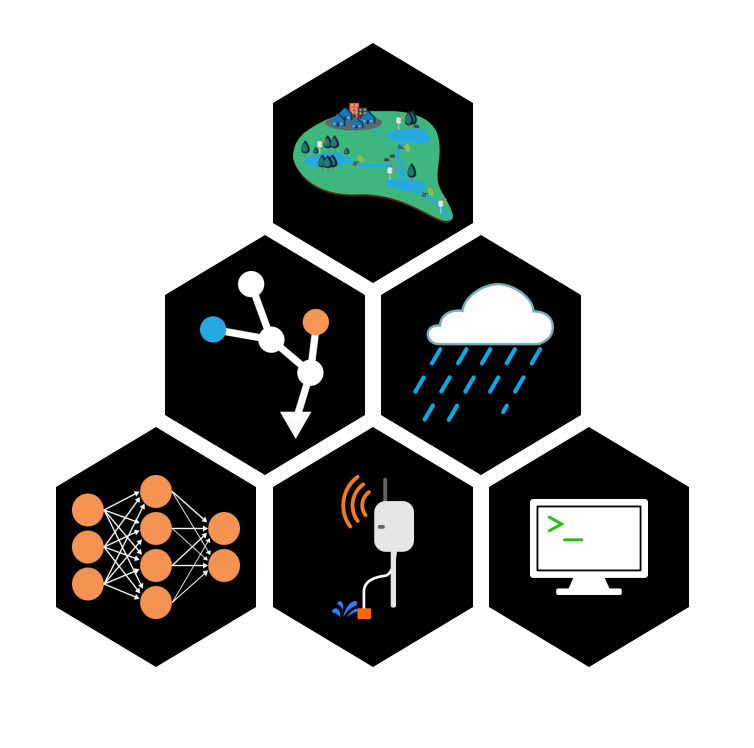
\includegraphics[width=8cm]{gfx/title_page.png} \\ \medskip

	\medskip
	\small{A dissertation submitted in partial fulfillment\\
	of the requirements for the degree of \\
        \myDegree \\
	(Civil Engineering)\\
        %\myFaculty \\
        in \myUni \\
July 2020 \\}

	\bigskip
	
	\spacedlowsmallcaps{Dissertation Committee}\\
	\myFaculty\\
	\myProf \\
	\myOtherProf \\
	\mySupervisor (Chair)\\


        \vfill

    \end{center}
  \end{addmargin}
\end{titlepage}

\thispagestyle{empty}

\hfill

\vfill

\noindent\myName: \textit{\myTitle,} \mySubtitle, %\myDegree,
\textcopyright\ \myTime

%\bigskip
%
%\noindent\spacedlowsmallcaps{Supervisors}: \\
%\myProf \\
%\myOtherProf \\
%\mySupervisor
%
%\medskip
%
%\noindent\spacedlowsmallcaps{Location}: \\
%\myLocation
%
%\medskip
%
%\noindent\spacedlowsmallcaps{Time Frame}: \\
%\myTime

\cleardoublepage%*******************************************************
% Dedication
%*******************************************************
\thispagestyle{empty}
\phantomsection
\pdfbookmark[1]{Dedication}{Dedication}

\vspace*{3cm}

\medskip

\begin{center}
    Dedicated to my family.\\ \smallskip
\end{center}

%\cleardoublepage\include{FrontBackmatter/Foreword}
\cleardoublepage%*******************************************************
% Abstract
%*******************************************************
%\renewcommand{\abstractname}{Abstract}
\pdfbookmark[1]{Abstract}{Abstract}
% \addcontentsline{toc}{chapter}{\tocEntry{Abstract}}
\begingroup
\let\clearpage\relax
\let\cleardoublepage\relax
\let\cleardoublepage\relax

\chapter*{Abstract}
\vspace{-0.5cm}
Rapid advances in wireless communication, embedded systems, and high-performance computing are promising the fusion of physical and digital water.
The next generation of stormwater systems --- equipped with wireless sensors and actuators --- will autonomously reconfigure themselves to prevent  flooding and achieve system scale objectives.
This vision of ``smart'' stormwater systems is not limited by technology, which has matured to the point where it can be ubiquitously deployed.
Instead, the challenge is much more fundamental and rooted in a system-level understanding of stormwater networks: \textit{once stormwater systems become highly instrumented, how should they be controlled to achieve the desired watershed outcomes?} This dissertation leverages statistical learning methods to begin closing fundamental knowledge gaps in the emerging field of smart water systems.
% Each chapter
% Second Chapter.
The second chapter of this dissertation addresses the lack of simulation tools for modeling pollutant interactions by introducing a new toolchain for coupling the existing hydraulic, hydrologic, and water quality models.
Using this toolchain, we demonstrate real-time control's potential for enhancing nutrient removal in a watershed.
% Real-time control's potential for enhancing nutrient removal in a watershed is demonstrated using this toolchain.
% Third Chapter 
In the third chapter, to characterize a watershed's controllability, a real-world case study is carried out using a wireless sensor-actuator network.
Through this study, the ability to precisely shape the hydrograph is quantified, illustrating the high level of granularity that can be achieved using real-time control. 
% Fourth Chapter 
Given that most state-of-the-art stormwater control algorithms require surrogate models or assume simplified dynamics, the fourth chapter introduces a Reinforcement Learning-based model-free algorithm for synthesizing stormwater controllers.
The efficacy of the algorithm is demonstrated via simulation, highlighting strong performance.
More importantly, a discussion is provided on the limitations of the approach, and a set of guidelines is presented for those seeking to apply Reinforcement Learning to stormwater control.
% Fifth Chapter
The fifth chapter in this dissertation introduces a Bayesian Optimization-based methodology for addressing the lack of knowledge relating to the uncertainty in stormwater control approaches and demonstrates its use for identifying robust control strategies.
% Sixth Chapter.
In the final chapter, an open-source Python library to facilitate the systematic quantitative evaluation of control algorithms is introduced.
This library provides a curated collection of stormwater control scenarios, coupled with an accessible programming interface and a stormwater simulator, to provide a standalone package for developing stormwater control algorithms.
% Two lines on the future and conclude.
The discoveries made in this dissertation, along with the algorithms and tools developed, seek to support the development of a new generation of autonomous stormwater infrastructure.
%foundation for
\endgroup

\vfill

%The fifth chapter in this dissertation introduces a Bayesian Optimization-based methodology for quantifying the uncertainties associated with control decisions and demonstrate its use for identifying robust control strategies.
%Quantifying these uncertainties enables us to identify the robust control strategies that can be implemented in a stormwater network.
%We demonstrate its effectiveness via a simulation-based evaluation and provide guidelines for adapting this approach for the control of stormwater systems.


\cleardoublepage%*******************************************************
% Publications
%*******************************************************
\pdfbookmark[1]{Publications}{publications}
\chapter*{Publications}%\graffito{This is just an early --~and currently ugly~-- test!}
%This might come in handy for PhD theses: some ideas and figures have appeared previously in the following publications:

%\noindent Put your publications from the thesis here. The packages \texttt{multibib} or \texttt{bibtopic} etc. can be used to handle multiple different bibliographies in your document.

Publications from this thesis. 

\begin{refsection}[ownpubs]
    \small
    \nocite{*} % is local to to the enclosing refsection
    \printbibliography[heading=none]
\end{refsection}

%\emph{Attention}: This requires a separate run of \texttt{bibtex} for your \texttt{refsection}, \eg, \texttt{ClassicThesis1-blx} for this file. You might also use \texttt{biber} as the backend for \texttt{biblatex}. See also \url{http://tex.stackexchange.com/questions/128196/problem-with-refsection}.

\cleardoublepage%*******************************************************
% Acknowledgments
%*******************************************************
\pdfbookmark[1]{Acknowledgments}{acknowledgments}

\begin{flushright}{\slshape
    We have seen that computer programming is an art, \\
    because it applies accumulated knowledge to the world, \\
    because it requires skill and ingenuity, and especially \\
    because it produces objects of beauty.} \\ \medskip
    %--- \defcitealias{knuth:1974}{Donald E. Knuth}\citetalias{knuth:1974} \citep{knuth:1974}
\end{flushright}



\bigskip

\begingroup
\let\clearpage\relax
\let\cleardoublepage\relax
\let\cleardoublepage\relax
\chapter*{Acknowledgments}
%Put your acknowledgments here.

%Many thanks to everybody who already sent me a postcard!

%Regarding the typography and other help, many thanks go to Marco
%Kuhlmann, Philipp Lehman, Lothar Schlesier, Jim Young, Lorenzo
%Pantieri and Enrico Gregorio\footnote{Members of GuIT (Gruppo
%Italiano Utilizzatori di \TeX\ e \LaTeX )}, J\"org Sommer,
%Joachim K\"ostler, Daniel Gottschlag, Denis Aydin, Paride
%Legovini, Steffen Prochnow, Nicolas Repp, Hinrich Harms,
%Roland Winkler, Jörg Weber, Henri Menke, Claus Lahiri,
%Clemens Niederberger, Stefano Bragaglia, Jörn Hees,
%Scott Lowe, Dave Howcroft, Jos\'e M. Alcaide, David Carlisle,
%Ulrike Fischer, Hugues de Lassus, Csaba Hajdu, Dave Howcroft, 
%and the whole \LaTeX-community for support, ideas and
%some great software.

%\bigskip

%\noindent\emph{Regarding \mLyX}: The \mLyX\ port was intially done by
%\emph{Nicholas Mariette} in March 2009 and continued by
%\emph{Ivo Pletikosi\'c} in 2011. Thank you very much for your
%work and for the contributions to the original style.


\endgroup

\cleardoublepage%*******************************************************
% Table of Contents
%*******************************************************
\pagestyle{scrheadings}
%\phantomsection
\pdfbookmark[1]{\contentsname}{tableofcontents}
\setcounter{tocdepth}{2} % <-- 2 includes up to subsections in the ToC
\setcounter{secnumdepth}{3} % <-- 3 numbers up to subsubsections
\manualmark
\markboth{\spacedlowsmallcaps{\contentsname}}{\spacedlowsmallcaps{\contentsname}}
\tableofcontents
\automark[section]{chapter}
\renewcommand{\chaptermark}[1]{\markboth{\spacedlowsmallcaps{#1}}{\spacedlowsmallcaps{#1}}}
\renewcommand{\sectionmark}[1]{\markright{\textsc{\thesection}\enspace\spacedlowsmallcaps{#1}}}
%*******************************************************
% List of Figures and of the Tables
%*******************************************************
\clearpage
% \pagestyle{empty} % Uncomment this line if your lists should not have any headlines with section name and page number
\begingroup
    \let\clearpage\relax
    \let\cleardoublepage\relax
    %*******************************************************
    % List of Figures
    %*******************************************************
    %\phantomsection
    %\addcontentsline{toc}{chapter}{\listfigurename}
    \pdfbookmark[1]{\listfigurename}{lof}
    \listoffigures

    \vspace{8ex}

    %*******************************************************
    % List of Tables
    %*******************************************************
    %\phantomsection
    %\addcontentsline{toc}{chapter}{\listtablename}
    \pdfbookmark[1]{\listtablename}{lot}
    \listoftables

    \vspace{8ex}
    % \newpage

%    %*******************************************************
%    % List of Listings
%    %*******************************************************
%    %\phantomsection
%    %\addcontentsline{toc}{chapter}{\lstlistlistingname}
%    \pdfbookmark[1]{\lstlistlistingname}{lol}
%    \lstlistoflistings
%
%    \vspace{8ex}
%
%    %*******************************************************
%    % Acronyms
%    %*******************************************************
%    %\phantomsection
%    \pdfbookmark[1]{Acronyms}{acronyms}
%    \markboth{\spacedlowsmallcaps{Acronyms}}{\spacedlowsmallcaps{Acronyms}}
%    \chapter*{Acronyms}
%    \begin{acronym}[UMLX]
%        \acro{DRY}{Don't Repeat Yourself}
%        \acro{API}{Application Programming Interface}
%        \acro{UML}{Unified Modeling Language}
%    \end{acronym}

\endgroup

%********************************************************************
% Mainmatter
%*******************************************************
\cleardoublepage
\pagestyle{scrheadings}
\pagenumbering{arabic}
%\setcounter{page}{90}
% use \cleardoublepage here to avoid problems with pdfbookmark
\cleardoublepage
%\part{Some Kind of Manual}\label{pt:manual}
%************************************************
\chapter{Introduction}\label{ch:introduction}
%************************************************
%************************************************
%************************************************
%What are stormwater systems and why are they needed and what is the problem?
Stormwater infrastructure is designed to mitigate the adverse effects of urbanization, including flooding and deterioration of watershed ecosystems~\cite{national2009urban, randhir2009urbanization}.
Stormwater systems reduce or eliminate these challenges by treating and transporting the accumulated stormwater runoff away from the urban environment and into a downstream water body~\cite{national2009urban}.
Existing stormwater systems are increasingly being stressed beyond their intended design~\cite{kerkez2016, national2009urban}.
The resulting symptoms manifest themselves in frequent flash floods\cite{LarisKarklisBefore-and-afterPost} and poor water quality in downstream water bodies\cite{Watson2016TheHypoxia}.
While these infrastructure systems can be rebuilt with larger storage capacity to keep pace with the evolving demands, such an undertaking might not be financially viable for most communities\cite{kerkez2016}.
Furthermore, stormwater systems are often designed and constructed in a piecemeal fashion.
Emerson et al.\ have demonstrated that such a localized approach is not guaranteed to improve the stormwater system's performance~\cite{Emerson2005Watershed-ScaleBasins}.
When small-scale solutions cannot be guaranteed to result in system-scale benefits,  new solutions are warranted.

\

%So how do we go about fixing it? : wireless sensing and control, but controlling this is not easy.
In lieu of new construction, one alternative would be to retrofit existing stormwater systems with sensors and controllers, so that these systems can be dynamically controlled in real-time to achieve the desired response\cite{kerkez2016, Mullapudi_Wong_Kerkez_2017}.
Such a vision is not limited by technology, which has matured to the point where it can be ubiquitously deployed\cite{Bartos_2018}.
Rather, the challenge is much more fundamental and rooted in a system-level understanding of environmental science.
Once stormwater systems become highly instrumented and controlled, how should they be operated to achieve desired watershed outcomes?

\

% What about other approaches from reservoir systems and why cant we use those methods?
The Water Resource Engineering community has extensively studied the control of water networks, and there is a significant volume of work focused on developing algorithms for the control of big reservoir systems~\cite{Haimes_1977,Labadie_2004,Yeh_1985,Reed_Hadka_Herman_Kasprzyk_Kollat_2013}.
However, much of these efforts have focused on large river basins, which change slowly and exhibit variable dynamics compared to urban stormwater networks~\cite{loucks2017water, te2010applied}.
Direct adoption of these existing methods for the control of stormwater systems is hindered by the fundamental scaling properties of water systems:
\begin{itemize}
	\item \textbf{Spatial properties}: Classical reservoir control methodologies formulate the control of water in the network of large storage nodes --- often separated by hundreds of miles --- as a linear (or convex nonlinear) optimization problem~\cite{Haimes_1977}.
As the water moves between these storage nodes, the impact of nonlinear wave dynamics becomes negligible and can be safely ignored.
However, given that the stormwater storage nodes are considerably smaller and are closer to each other, the impact of wave dynamics is significant and has to be incorporated into the decision process. 
\item \textbf{Temporal properties}: Given the long decision time horizons\footnote{In the order of months.}~\cite{You_Cai_2008}, the influence of nonlinearities in hydrological and hydraulic phenomena, such as runoff generation and flow of water through outlet structures, is often ignored or approximated as linear systems in reservoir control.
Stormwater systems operate on a much smaller time horizon (in the order of minutes)~\cite{lund2018}.
At such smaller time scales, the nonlinearities in hydrological and hydraulic phenomena are significant and have to be accounted into control decisions.
\end{itemize}
Relatively recently, there have been works investigating the use of evolutionary algorithms~\cite{Reed_Hadka_Herman_Kasprzyk_Kollat_2013, maier2014,Bessler_Savic_Walters_2003} for reservoir control, and these algorithms are increasingly being used for the control of stormwater systems~\cite{shishegar2018optimization,lund2018}.

\


The state-of-the-art in stormwater control  can be broadly classified under two categories: (1) Control algorithms reliant on parametrized models (e.g.\ model predictive control) for identifying control actions~\cite{Wong_Kerkez_2018, Ocampo-Martinez_2015,joseph2014hybrid, Sun_2020, lund2020cso}. (2) Search-based algorithms (e.g.\ evolutionary optimization algorithms) that exhaustively simulate physical models for identifying control actions~\cite{shishegar2018optimization,sadler2019, lund2018, Rjeily_2018, Meneses_2018, vezzaro2014}.
Though these control algorithms have been applied for localized control in stormwater systems\footnote{e.g.\ maintaining constant water levels and flows in individual basins.}, their investigation in the context of coordinated control and targeted removal of pollutants has been limited.
To fully realize the potential of the stormwater infrastructure and to safeguard our water bodies, we need to synthesize control algorithms that are able to coordinate the response of many distributed control assets in the network, while simultaneously achieving a diverse set of water quality and flow objectives. 
Technologically, we are at a point where we can monitor and control these assets in real-time, but the development of control algorithms is hampered by a number of fundamental knowledge gaps:
\begin{itemize}
	\item We do not know how to design control algorithms that can target pollutants in stormwater runoff, nor do we have the simulation tools necessary for such studies.
	\item We do not know to how to characterize the controllability of an urban watershed, especially in the context of water quality.
	\item We do not yet know how to synthesize reliable control algorithms for distributed stormwater assets without making explicit dynamical assumptions (e.g.\ linearity).
	\item We do not know how to quantify the uncertainty of rainfall in algorithms used in the control of stormwater systems.
	\item We do not have open platforms for the systematic quantitative evaluation and comparison of different control algorithms.
\end{itemize}

My dissertation, leveraging statistical approaches, addresses these knowledge gaps to support algorithms that control stormwater systems. This work is divided into the following five chapters:

\begin{itemize}
	\item \textbf{Chapter-2}: This chapter introduces a modular framework for simulating real-time control in stormwater systems and demonstrates control's effectiveness in enhancing nutrient removal.
	\item \textbf{Chapter-3}: This chapter demonstrates the use of a real-world wireless sensor-actuator network for precisely shaping streamflows in a stormwater network.
	\item \textbf{Chapter-4}: This chapter introduces a Reinforcement Learning-based algorithm for the control of stormwater systems and evaluates its applicability across a diverse set of stormwater scenarios.
	\item \textbf{Chapter-5}: This chapter introduces a Bayesian Optimization-based algorithm for the automated control of stormwater networks and demonstrates this algorithm's ability to quantify rainfall uncertainties associated with the control decisions. 
	\item \textbf{Chapter-6}: This chapter introduces an open-source Python library to facilitate the systematic quantitative evaluation of stormwater control algorithms.
\end{itemize}
 

\section{Chapter 2: Building a theory for smart stormwater systems}

Retrofitting existing stormwater systems with wireless sensors and controllers will enable real-time control of flooding, stream erosion, and pollutant treatment. 
The adoption of these smart systems is not limited by the technology, which has matured to a point where it can be deployed ubiquitously, but rather by our understanding of system-scale environmental science.
This demands the development of a theoretical framework for smart stormwater systems.
However, given the limitations in the existing stormwater simulation tools, we cannot adequately model pollutant transformations on a watershed scale.
This fundamentally limits our ability to synthesize and evaluate system-scale control algorithms. 
In the second chapter of this dissertation, we present a modeling framework for simulating the real-time control of stormwater systems and pose the requirements for developing a theory of smart stormwater systems.

\

% Methodology
A comprehensive literature review is offered in the chapter, highlighting primarily that existing stormwater simulation tools can be broadly grouped into two categories: those that focus on hydrology (on a watershed scale)\cite{Rossman2010Storm5.1} and those that focus on water quality (at individual sites)\cite{Langergraber2009CWM1:Wetlands}.
This often forces a trade-off between comprehensively modeling system-level hydrology and pollutant treatment.
We propose a modular approach that integrates these existing models under a common simulation framework, rather than incorporating the desired functionality in a single unified model.
This choice was motivated by the desire to ensure compatibility with the existing tools and to provide the researchers with the flexibility of incorporating their custom models into the framework.
We demonstrate the use of this framework on two simulated case studies, which focus on nutrient treatment in an urban watershed.

\

% Contribution
This chapter's main contribution is demonstrating the use of real-time control for enhancing nutrient removal in stormwater systems.
The modular simulation framework developed in this chapter has been the foundation for the control algorithms and the simulation tools developed in this dissertation. 

\section{Chapter 3: Shaping streamflow in real-time using a sensor-actuator network}

The primary objective of this chapter is to illustrate how data from a stormwater sensor network can be leveraged to precisely shape the hydrographs at the outlet of an urban watershed.
Leveraging a wireless sensor-actuator network in Ann Arbor~\cite{Bartos_2018}, we characterize the travel-times and magnitudes of flows resulting from a control system's actions.
Based on this characterization, we formulate a series of experiments to illustrate how such an approach achieves flow control objectives.
We create a flat hydrograph using a single control asset to illustrate the use of water level data in maintaining system-level flows below a desired stream erosion threshold.
We also demonstrate the coordinated control of two controllable stormwater assets for shaping streamflow at the outlet of the watershed.

\

The third chapter demonstrates the characterization and control of an urban watershed using wireless sensor-actuator networks. 
To the best of our knowledge, the study presented in this chapter is the first-ever study to demonstrate the use of coordinated control strategies for achieving system-scale objectives in a real watershed.

\section{Chapter 4: Deep Reinforcement Learning for the control of stormwater networks}

Presently, state-of-the-art control of stormwater falls under classic linear model predictive control (MPC)\cite{Wong_Kerkez_2018}.
While this enables us to analytically evaluate the stability, robustness, and ensure performance guarantees, the approach demands a number of approximations, assumptions, and a high level of user expertise\cite{Wong_Kerkez_2018, Ocampo-Martinez_2015, joseph2014hybrid}.
Furthermore, real-world urban watersheds are prone to experiencing pipes blockages, sensor breakdowns, and other adverse conditions\cite{national2009urban}.
Adapting and re-formulating linear control models to such non-linear conditions is difficult.
The constraints of linear approximations and the need for adaptive control algorithms open the door to exploring other control methodologies, such as Reinforcement Learning (RL)~\cite{Sutton98}.
In this chapter, we introduce the first ever evaluation of RL for the control of stormwater systems.

\

We analyze the feasibility of RL-based control of stormwater systems by formulating a series of simulation-based experiments.
The controller's sensitivity to reward function formulation is evaluated by training the controller on a single basin using five different reward functions and analyzing final performance.
The scalability of the approach is analyzed by training the controller on a network of three interconnected basins.
The robustness of the controller formulation to the choice of neural network architecture is also evaluated.
%We then analyze the trained controller's performance on a spectrum of storm events to quantity the benefits of the proposed control approach.


\

The chapter's main contribution is the formulation and implementation of an RL-based algorithm for the control of urban stormwater systems.
We evaluate the RL-based control approach's performance across a range of storm inputs and network complexities to demonstrate its effectiveness and limitations.
We also provide a fully open-sourced implementation of the control algorithm to promote transparency and permit the method's direct application to other systems.


\section{Chapter 5: Bayesian Optimization for shaping stormwater flows}

Early evaluations of Reinforcement Learning-based control have suggested that controllers often maintain nearly constant control actions (valve positions) throughout a storm event~\cite{Mullapudi_Lewis_Gruden_Kerkez_2020}.
This may mitigate the need for real-time control, as one could preset the control action ahead of a storm without needing to change it in real-time. 
While such an approach considerably simplifies the control problem, the solution space is still large enough for conventional search approaches to be efficient.
Furthermore, unlike feedback control, in this proposed planning based control approach, the controller cannot alter its course if its actions result in an unintended response. 
Hence, planning for the possible uncertainties and choosing a risk-averse control strategy becomes essential.
To address these challenges, in this chapter, we introduce a Bayesian Optimization-based methodology for identifying the optimal control actions and quantifying their associated uncertainties.

\

We investigate the feasibility of the proposed approach by analyzing its ability to identify optimal control decisions that realize the desired response across stormwater networks.
We evaluate its computational efficiency by comparing its performance to a Genetic Algorithm, a widely used search-based stormwater control approach.
Finally, we propose a methodology for extending Bayesian Optimization's ability to quantify rainfall uncertainty associated with the control decisions.

\

This chapter's main contributions include a methodology for shaping stormwater flows and an algorithm that establishes bounds on the controller's performance by quantifying impacts of rainfall uncertainty.
We also provide an open-source implementation of the controller that can be applied to virtually any stormwater network for which a physical model exists.

\section{Chapter 6: A simulation sandbox for the development and evaluation of stormwater control algorithms}\sectionmark{Chapter-6: \texttt{pystorms}}

Over the past decade, there has been a significant amount of work in the development of real-time control algorithms for stormwater systems~\cite{shishegar2018optimization, lund2018, Ocampo-Martinez_2015}.
Most, if not all, of the proposed algorithms were evaluated on specific stormwater networks and perturbed by a particular set of storm events~\cite{lund2018}.
Many of the underlying models and parameterizations have not been made accessible to the broader research community~\cite{lund2018, Rimer2019}.
This limits the reproducibility of the work and creates a barrier for comparing the performance of these algorithms across networks under various storm conditions.
While there have been studies qualitatively comparing the performance of various control approaches~\cite{shishegar2018optimization}, Bors\'{a}nyi et al.\cite{Borsanyi2008} and others\cite{Schutze2017} recognized the need for a more quantitative evaluation for understanding the limitations and strengths of the proposed control strategies.

\

This chapter addresses these challenges by creating an open-source Python library that provides a collection of anonymized storm\-water networks and event drivers, curated as scenarios for facilitating the quantitative evaluation of control algorithms. These scenarios represent a diverse set of flooding, water quality, and flow control objectives that might be encountered in a real watershed.
These scenarios are coupled with an accessible programming interface and a stormwater simulator to provide a stand-alone library for developing stormwater control algorithms.
Furthermore, a web-page\footnote{\href{https://www.pystorms.org}{pystorms.org}} with tutorials is created to act as a resource for helping researchers get started with the real-time control of stormwater systems.

%************************************************
\chapter{Building a Theory for Smart Stormwater Systems}\label{ch:theory}
%************************************************
Rapid advances in sensing, computation, and wireless communications are promising to merge the physical with the virtual.
Calls to build the ``smart'' city of the future are being embraced by decision makers.
While the onset of self-driving cars provides a good example that this vision is becoming a reality, the role  of information technology in the water sector has yet to be fleshed out.
These technologies stand to enable a leap in innovation in the distributed treatment of urban runoff, one of ourlargest environmental challenges. 

\

Retrofitting stormwater systems with sensors and controllers will allow the city to be controlled in real-time as a distributed treatment plant.
Unlike static infrastructure, which cannot adapt its operation to individual storms or changing land uses, ``smart'' stormwater systems will use system-level coordination to reduce flooding and maximize watershed pollutant removal. Given the sheer number of storm water control measures in United States, even a small improvement to their performance could lead to a substantial reduction in pollutant loads.
Intriguingly, such a vision is not limited by technology, which has matured to the point at which it can be ubiquitously deployed. 
Rather, the challenge is much more fundamental and rooted in a system-level understanding of environmental science.
Once stormwater systems become highly instrumented and controlled, how should they actually be operated to achieve desired watershed outcomes?
The answer to this question demands the development of a theoretical framework for smart stormwater systems. 
In this paper we lay out the requirements for such a theory.
Acknowledging that the broad adoption these systems may still be years away,  we also present and evaluate a modeling framework to allow for the simulation of smart stormwater systems before they become common place. 
Recent urban floods~\cite{Frosch2016}, many of which are driven by flashy events and inadequately sized infrastructure, are all too common example that aging stormwater infrastructure is struggling to keep pace with a dynamic and changing climate. 
While flood control often emerges as one of the most promising application areas, to illustrate the flexibility of smart stormwater systems this paper will focus on the impacts to urban water quality.


\section{Do best local practices achieve the best global outcomes?}

Pollutants in runoff are threatening the health of downstream ecosystems, as evinced by harmful algal blooms, such as those on Lake Erie~\cite{Michalak2013Record-settingConditions} and the Chesapeake Bay~\cite{powledge2005chesapeake,Boesch2001ChesapeakeAgriculture}.
Simultaneously, ``dry'' regions of the country are struggling to find new and clean sources of water.
By some estimates, the capture of stormwater in Los Angeles~\cite{Geosyntec2014} and San Francisco~\cite{Garrison2014StormwaterCalifornia} could offset the water used by these cities.
This, however, requires at least some level of treatment to ensure that captured stormwater is safe for direct use or aquifer injection.
In the face of these challenges, novel solutions for stormwater management are needed.

\

Reductions in hydraulic or pollutant loads are commonly achieved via a set of distributed stormwater solutions~\cite{Hamel2013Source-controlReview, Burns2012HydrologicReform}, such as ponds or treatment wetlands.
Our body of knowledge on the treatment potential of these systems is extensive, showing that significant water quality and hydraulic benefits can be achieved at the level of individual sites~\cite{Stanley1996PollutantPond,Carleton2000PerformanceRunoff}.
Most recently, an exciting and growing research area has formed around smaller-scale and more distributed Green Infrastructure (GI) solutions, such as green roofs or bioswales\cite{Benedict2006GreenCentury}.
Most of these solutions are grouped under the broader umbrella of Best Management Practices\cite{Urbonas1994ASSESSMENTTECHNOLOGY} (BMPs) or Storm Water Control Measures (SCMs)\cite{Cizek201340}.

\

Given the aggressive adoption of these stormwater practices, rarely is the question asked: Does doing the ``best'' at a local scale translate to doing the best at the watershed scale? Research on this question is limited\cite{Petrucci2013DoOutcomes,Sage2015StormwaterPractices,Petrucci2014UrbanHow}, but paints a cautionary picture.
Unless designed as part of a coordinated, city-scale solution, a system of SCMs may actually worsen watershed-scale outcomes.
For example, unless coordinated at design-time, hydrographs from individual SCMs
may add up to cause larger downstream flows compared to the same watershed
without these SCMs\cite{Emerson2005Watershed-ScaleBasins}.
This, in turn, can lead to increased stream erosion and re-suspension of sediment-bound pollutants.
More examples can be given, but there is an urgent need to investigate the
scalability of SCMs and to ensure that their functionality is tuned in the context of the broader stormwater system. 

\

Even if system-level optimization is used to determine the placement of SCMs\cite{Ciou2012OptimizationWatershed,Zhen2004OptimalScale}, it is difficult to guarantee that the overall system will perform as designed.
The sheer variability in rainfall\cite{Chaubey1999UncertaintyRainfall}, seasonal pollutant loadings\cite{Ouyang2006AssessmentQuality}, and broader land use changes\cite{Goonetilleke2005UnderstandingManagement} will always push stormwater systems beyond their intended design or the ``average'' storm\cite{DepartmentofEnvironmentalProtection2006PennsylvaniaManual}.
As such, it becomes imperative to find a way to adapt to these uncertain disturbances.
One solution relies on real-time sensing and control.
By equipping stormwater elements with control valves, which can be operated in real-time based on sensor readings, the overall performance of the entire system can be adapted to achieve watershed-scale benefits (Figure.\ref{fgr:vision}a). 

%%------------------RTC studies ---------------
\subsection{Existing studies on real-time control}

The bulk of existing literature on real-time control of stormwater SCMs focuses on water quality and hydraulic impacts at individual sites, particularly ponds and basins.
These studies assume that the outlet of a BMP has been retrofitted with a remotely controllable gate or valve.
By strategically controlling outflows before or during storm events, internal volumes can be modified and hydraulic retention time (HRT) can be increased.
Jacopin et al.\cite{Jacopin2001OptimisationBasins} demonstrated that detention basins, designed for flood control, can reduce sediment-based pollutant loading (57\% decrease) in downstream water bodies by simply opening and closing a valve.
Middleton et al.\cite{Middleton2008WaterBasin} analyzed the water quality response of a controlled detention basin, observing up to a 90\% improvement in TSS and ammonia-nitrate removal.
Recent studies\cite{Muschalla2014Ecohydraulic-drivenBasins,
  Gaborit2013ImprovingForecasts,Gaborit2015ExploringPonds} in Quebec, Canada,
proposed a rule-based control logic for a pond, based on rainfall forecasts, to
maximize retention time and  reduce hydraulic shocks to the downstream water
bodies. The authors observed a 90\% improvement in TSS retention. A
comprehensive review of these and other studies is summarized in Kerkez et al.\cite{Kerkez2016SmarterSystems}, along with additional information on how these solutions are deployed in the field. 
While these studies demonstrate significant potential to improve water quality at the scale of individual sites, the mechanisms behind the removal of pollutants in controlled SCMs remain a research challenge. This is particularly true in the removal of dissolved pollutants, such as ammonia and nitrate. Furthermore, the scalability of  real-time control must be evaluated to ensure that local benefits do not overshadow watershed-scale benefits. 


\begin{figure}
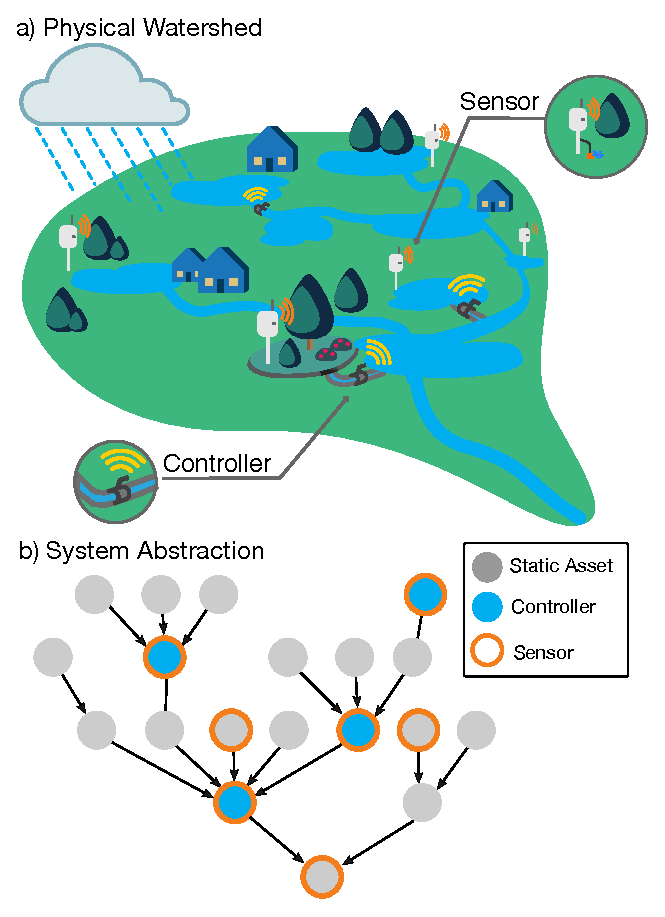
\includegraphics{gfx/Chapter-1/k-drawing.eps} 
\caption{Application of control and optimization methods to the real-time operation of stormwater systems will be made possible by abstracting physical models to system-theoretic representations.}
\label{fgr:vision}
\end{figure}


Since the 2000 European Union's Water Framework Directive \cite{TheEuropeanParliamentandthecouncilofEuropeanUnion2000DirectivePolicy} there has been an increasing emphasis on integrated, system-level control of sewer water distribution systems.
The resulting control strategies vary in complexity\cite{Benedetti2009AScale,Seggelke2013ImplementationWilhelmshaven,Fiorelli2013OptimisedFunction}  and have since been implemented in a number of urban water networks\cite{Mollerup2016ControllingCities}.
Applying these methods to distributed stormwater solutions introduces a new set of challenges, however. Unlike in well-maintained sewer networks, the exposed and distributed  nature of stormwater systems introduces complexities associated with the urban hydrologic cycle, such as infiltration, evaporation, soil moisture and groundwater dynamics. Furthermore, one major function of stormwater systems relates to the  distributed control of  a large variety of solid, dissolved and emerging pollutants. Control of sewer networks is often targeted at volume control to mitigate sewer overflows or overloading treatment plants. As such, much work remains to be conducted on investigating how these methods can be applied to the distributed control of SCMs. 



\section{Toward a framework for smart stormwater systems}
 
Many methods have been developed by the operational research and control theory communities to optimize the operation of networked systems\cite{Sheffi1984UrbanNetworks,Astrom2006FeedbackEngineers}. Given their inherent non-linearity and complexity, existing stormwater models are not compatible with these tools. To that end, our knowledge of treatment processes and the physical nature of stormwater systems must first be embedded in a system-theoretic framework (Figure.\ref{fgr:vision}b). Such a formal and mathematical approach will be crucial toward developing a system-level understanding of stormwater. Not only will this framework help to control future stormwater systems, but it will also create a foundation upon which to answer critical questions, such as: How many controllers are needed and where should they be placed to achieve best system-level benefits?  Consequently, how many sensors are needed and where should they be placed to help the control system achieve these objectives? 

Until sensors and controllers become ubiquitously deployed across stormwater systems, which may take years to accomplish, there is enough domain knowledge embedded in existing models to begin answering these questions through simulation. 


%%simulation framework
\subsection{Limitations of existing simulations approaches}
Existing stormwater models can be broadly grouped into two categories: those
that focus on hydrology (including hydraulics) and those that focus on water quality. The former range across simple routines, such as Muskingum routing\cite{Brunner1991ANetworks} and the Rational Method\cite{Chin2000Water-resourcesEngineering}, to more complex hydrodynamic models that solve the St.Venant's equation, such as popular packages like SWMM\cite{Rossman2010Storm5.1} and HEC-RAS\cite{Brunner2016HECManual}. The latter, which include models such as HYDRUS\cite{Rizzo2014ModellingHYDRUS-CWM1,Palfy2014TheData} and FITOVERT\cite{Giraldi2010FITOVERT:Wetlands},  are used to simulate treatment processes within individual sites, such as wetlands and green infrastructure. The coupling of the two approaches often yields  
While some packages support extended features that model both hydrology and
storm water quality, much work needs to be conducted to improve their
accuracy. This often forces a trade-off between
comprehensively modeling system-level hydrology or local-level treatment.


Pollutant removal in stormwater is a highly complex and dynamic process. The rate at which pollutants undergo transformation is dependent upon the pollutant-type and its interaction with a given stormwater element (oxygen concentrations, soil types, biomass, settling times, water temperature, etc). Given the complexity of these interactions, popular hydraulic models, such as SWMM, MUSIC\cite{Wong2002AConceptualisation} and SUSTAIN\cite{Lai2007SUSTAINWATERSHEDS} often approximate pollutant treatment using first order decay models\cite{Kadlec2008TreatmentWetlands}:
\begin{equation}
	\frac{dC}{dt}=-kC
\end{equation}
where the concentration $C$ of a pollutant is assumed to decrease exponentially following a decay coefficient $k$. While this may be sufficient for approximating the settling dynamics of sediment-bound pollutants, it does not capture the nuanced and complex transformation of dissolved compounds. This often leads to treating the hydraulic retention time (HRT) as the main proxy for water quality. 

To that end, a number of approaches have been developed to extend first order decay models to account for variations in background concentration\cite{Shepherd2001Time-DependentConstr}, temperature\cite{Kadlec2008TreatmentWetlands}, loading rates\cite{Mitchell2001AlternativeKinetics} or mixing conditions\cite{Persson2003HowPonds,Wong2006ModellingApproach}. A number of process models have also been developed, applying knowledge from treatment plant operations to stormwater\cite{Langergraber2008ModelingReview}. Langergraber et al.\cite{Langergraber2009CWM1:Wetlands,NterLangergraber2005ModelingWetlands} used finite element analysis to model pollutant transformations in  subsurface flow wetlands. While these more comprehensive water quality models are highly promising, their ability to simulate system-level treatment remains to be explored.

Given the need to develop a better understanding of the system-level transport and treatment of stormwater, there is a need to couple existing hydraulic and water quality models. 

%%------------------Simulation framework ------------------ 


\section{Simulating controlled systems}
The real-time operation of gates and valves introduces dynamics that impact hydraulics and water quality.
To that end, the biggest limitation of existing models is their ability to simulate the system-wide impacts of real-time control.
This includes the ability to dynamically route flows based on a variety of desired control actions, as well as the capacity to simulate a variety of pollutant buildup, washoff, and non-steady state treatment dynamics. 
While models such as SWMM do have some rudimentary control capabilities, the built-in control logic is limited to site-level control (e.g.\ maintaining levels or flow in a pond)\cite{Rossman2010Storm5.1}.
Advanced features, such as system-level control, optimization, or the ability to control around external factors (such as weather forecasts) are not yet implemented\cite{Ria2016MatSWMMSystems}. 

While it would be possible to extend an existing model to capture all this functionality, the effort would be significant. To that end, we contend that a coupled modeling approach\cite{Goodall2011ModelingParadigm}  will be the most flexible way to accomplish this. By coupling models, rather than translating their features in  into one large model, it becomes possible to construct a modeling chain whose complexity varies based on the scientific or management question that needs to be answered. More importantly, if individual models undergo updates by their respective domain experts, these new features would become available to the coupled model as well without much implementation overhead. 

\begin{figure}
\centering
  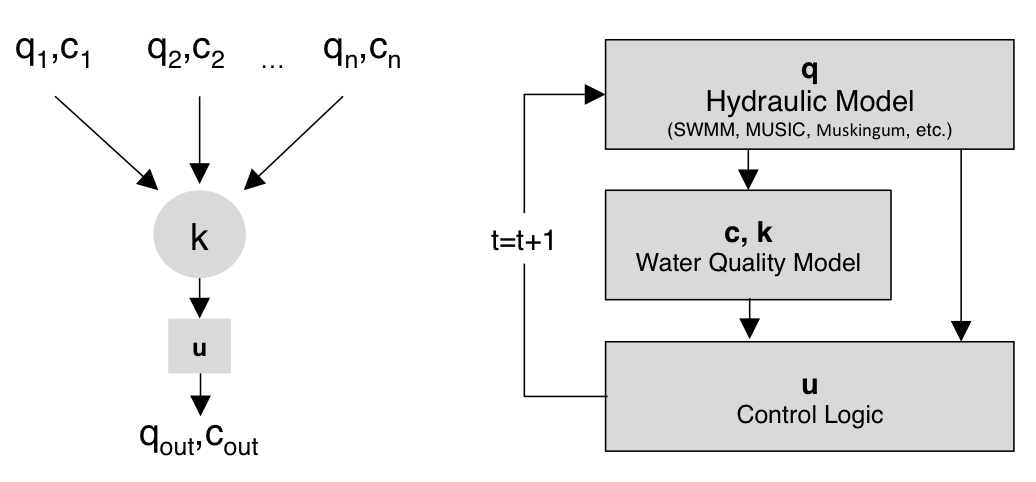
\includegraphics[width=\linewidth]{gfx/Chapter-1/coupled_model.png}
  \caption{Each element in the broader stormwater system can be modeled in a step-wise fashion that simulates hydraulic, water quality and control dynamics.}
\label{framework}
\end{figure}

In our coupled modeling approach (Figure\ref{framework}), each element in the
broader stormwater system can be represented as a storage node, which receives
inflows $q_1,q_2,\ldots,q_n$ from upstream nodes, each of which has a corresponding concentration $c_1,c_2,\ldots,c_n$ for a pollutant of interest.
The node has an outflow $q_{out}$ which, unlike in static hydraulic infrastructure, is governed by a real-time control action $u$. 
A treatment potential $k$ governs the removal or transformation of the pollutant based on a number of hydraulic and water quality states.
 
Given that control actions change the hydraulic behavior, which in turn affects the treatment of the pollutants, it becomes necessary to implement a modeling cycle that couples these processes in an interconnected, step-wise fashion. 
In our implementation, the hydraulic simulation can be carried out by any number of hydraulic models, ranging from simple hydraulic routing schemes, to more complex models such as SWMM or MUSIC.
Outputs from the hydraulic model are fed to the water quality model, which, depending on the pollutant of interest, can range from simple first-order process-based methods to more complex finite-element models.
Finally, the control module processes the outputs from the hydraulic and water quality models.
Based on the objective, which can depend on the states of multiples elements in the overall systems, it sets the discharge rate $q_{out}$  by closing or opening the outlet.
The benefits of the coupled approach relate to its flexibility since individual elements can be connected together to represent highly complex stormwater networks.

%%%%%-----------------case studies ------------------


\section{Simulated Studies}

To illustrate the potential benefits that can be achieved through
  real-time stormwater control, we applied the proposed simulation framework to
  two simulated case studies, which were inspired by our current research
  efforts in the Midwestern United States. Multiple sites are currently being
  retrofitted for control  and will be compared to these simulations in the
  coming years. The analysis was targeted on nitrate removal since most of the
  existing literature focuses on hydraulic control or sediment-bound
  pollutants.

\begin{enumerate}
	\item  Local scale: The first study investigated the impacts of real-time control to nitrate removal in a single stormwater pond.
    \item System scale: The second study evaluated how nitrate removal can be coordinated between a system of controlled stormwater elements.
\end{enumerate}

\subsection{Model Implementation}
Given the scope of the use cases, a simple flow balance module was sufficient to simulate the hydraulic behavior of each element. The change in water volume was modeled as the difference between inflows and outflows, which could be used to calculate the water height $h$ in each element based on its area $A$. Outflows from each element were proportional to the instantaneous pressure head, unless the element was controlled, in which case it was assumed that outflow can be set such that:

\begin{equation} \label{outflow}
 0 \leq  q_{out}  \leq \sqrt{2  g  h}
\end{equation}

Inflow into upstream elements was based on a hydrograph  that was directly measured at one of our study sites in Ann Arbor, Michigan (Figure.\ref{fgr:local_control}). Overflows were simulated in the case that the storage volume was exceeded. For simplicity, infiltration was assumed to be negligible in the study sites. 

A water quality model was developed to simulate nitrogen removal in each
stormwater element. While nitrogen removal processes are complex, we can
simplify their function for this example by assuming that the removal of nitrogen in stormwater ponds and wetlands occurs through two primary pathways: nitrification (conversion of ammonia to nitrate) and de-nitrification (conversion of nitrate to nitrogen gas)\cite{Kadlec2008TreatmentWetlands, Reddy1989Nitrification-DenitrificationWetlands}.  Nitrification is an aerobic process (oxygen acts an electron acceptor), while denitrification is anoxic (nitrate as electron acceptor). While denitrification requires sufficient biomass, it is often not limited by this requirement since plants, grass and other sources of carbon are readily present in stormwater ponds and wetlands\cite{White2009BiogeochemicalWetlands}. 
As such, oxygen availability becomes a critical factor in nitrogen removal. This can readily be tuned through hydraulic control since retention can be used create anaerobic conditions. 

We constrained our case studies by focusing only on denitrification, assuming that the majority of nitrogen entering our system was in the form of nitrate. While ammonia is present in some stormwater systems, prior measurement of our study sites, as well other literature\cite{Kadlec2008TreatmentWetlands}, indicated a nitrate-dominated runoff. 
Future studies will investigate the more complex dual-pathway conversion. 
A synthetic time series for Nitrate inflow concentrations was generated to simulate loads to upstream elements. 
This was achieved by assuming a rough correlation between flow and nitrate (2 $mgL^{-1}/m^3s^{-1}$), which was based on prior measurements\cite{Kerkez2016SmarterSystems}.

The water treatment for each element was simulated using a continuously stirred tank reactor (CSTR) representation, which is commonly used to simulate similar processes in wastewater treatment plants\cite{Henze2000ActivatedASM3}.
Given the dynamic flow conditions that result from real-time control, a closed-form solution that is based on hydraulic residence time does not adequately capture the change in concentration of the pollutant.
As such, it becomes necessary to expand into a complete CSTR mass-balance relation\cite{Alvord1996AtrazineWetlands,Kadlec2001PhosphorusWetlands,Munson2002ModelArea} to model the concentration $C$ of the dissolved pollutant:

\begin{equation} \label{cstr}
  \frac{dc}{dt}  V + \frac{dv}{dt}  C = q_{in}  C_{in} - q_{out}  C - k  C  V
\end{equation}

At each time step, the CSTR module communicates with the hydraulic module to update the hydraulic states $( \frac{dV}{dt}, V , q_{out} \ and \ q_{out})$. The transformation rate $k$ is computed at each time step based on the hydraulic conditions of the stormwater element. Specifically, denitrification can  begin once the oxygen concentration at the soil-water interface drops below a minimum threshold (following a first-order decay assumption). Once this occurs, a constant removal rate $k$ is activated. After the element drains, soil is exposed to the air and must be submerged before denitrification can begin again. As such, the model assumes that cumulative denitrification is maximized when the water is in contact with the most anaerobic soil area. 

All simulations were implemented in MATLAB Simulink\cite{TheMathWorksInc.MATLAB} using a fixed time step solver (ode8 Dormand-Prince\cite{Dormand1980AFormulae}) at 5 minute intervals. 
The step-wise coupled modeling approach was implemented by representing each  each module (hydraulic, water quality, and control) as an individual Simulink object (Figure.\ref{fgr:simulink}). All of the source code, inputs and implementation details are attached to this paper as supplementary material.

\begin{figure}
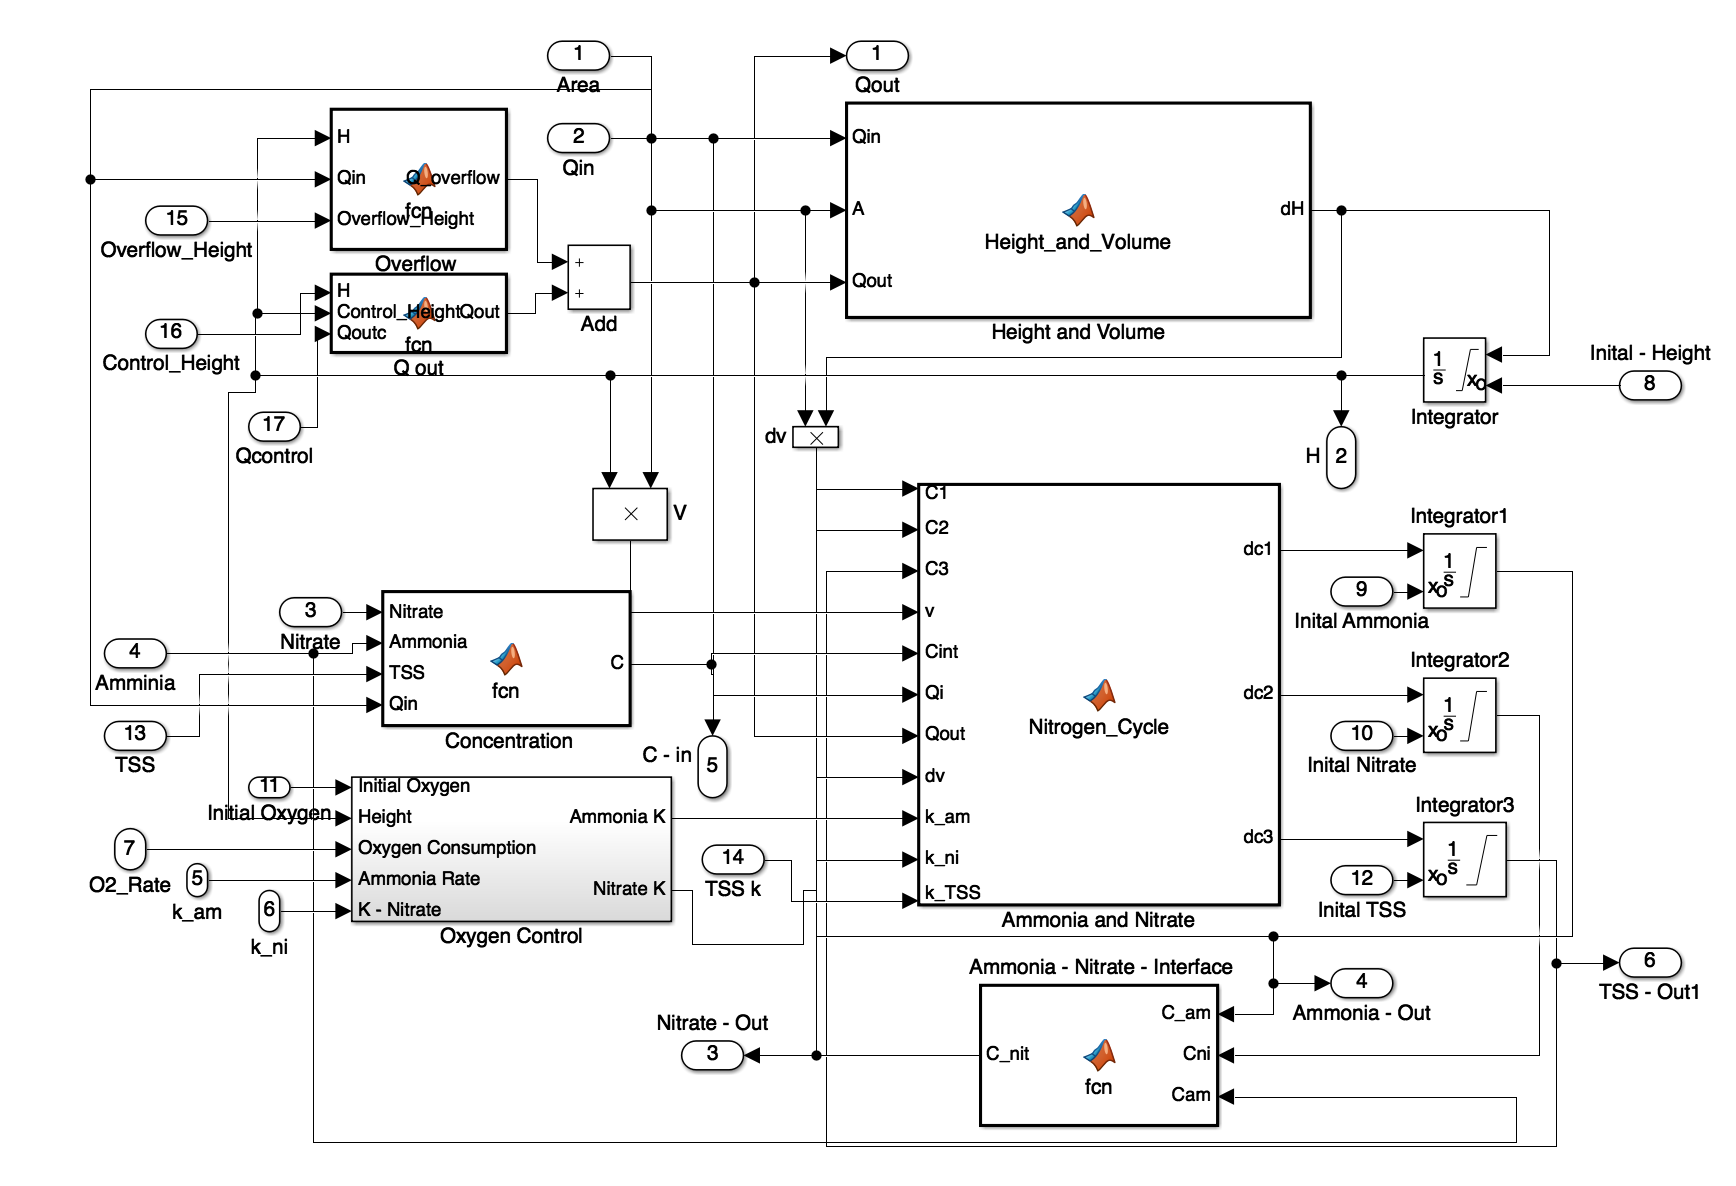
\includegraphics[width=\linewidth]{gfx/Chapter-1/Model_Individual.png}
  \caption{MATLAB Simulink implementation of the first case study. The overall model executed in a step-wise fashion and couples stand-alone hydraulic, water quality, and control models.}
\label{fgr:simulink}
\end{figure}

%--------------------------- Local CONTROL -----------------

\subsection{Case Study 1: Local Control}

\begin{figure}
\centering
  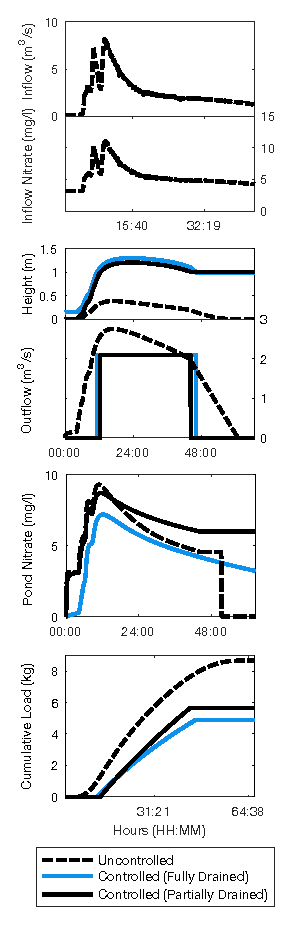
\includegraphics{gfx/Chapter-1/local.eps}
  \caption{Impact of real-time control to hydraulic behavior and nitrate treatment, showing inflow concentrations (top panel), pond water height and outflows (second panel), nitrate concentrations inside the pond (third panel), and cumulative nitrate loads exiting the pond (bottom panel).}
\label{fgr:local_control}
\end{figure}

The first case study is motivated by the objective of controlling a single stormwater basin, which was originally designed for flood remediation as a detention pond (flow-through).  The model parameters and physical attributes are provided in the appendix of this paper. In its original configuration the pond merely serves to attenuate peak flows, with little emphasis on water quality. By equipping this pond with a control valve, its original functionality can remain unaffected during large storms by simply keeping the valve open.  Major water quality benefits can arise, however, by controlling this pond during smaller and more frequent events. 

When enabled, the control algorithm keeps the valve closed and only opens it if the water height exceeds 1.0 m to prevent the pond from overflowing. As a further constraint, when the height exceeds 1.0 m the valve is modulated to ensure that outflows do not exceed $2m^3s^{-1}$, which is the threshold at which downstream sediments are assumed to be re-suspended. Two variations of the control algorithm are also evaluated. The first strategy completely drains the pond before a rain event, thus maximizing captured volumes. Based on the magnitude of the rain event (assumed to be known through a weather forecast), the second strategy only partially drains the pond, maximizing the anaerobic conditions at the soil-water interface and thus speeding up denitrification of the inflows. In this case study, the  height of the partially drained configuration was set to 0.15 m, assuming that this height would be sufficient to maintain the saturated conditions and prevent the diffusion of oxygen into soil \cite{Reddy1989Nitrification-DenitrificationWetlands}. 

Compared to the uncontrolled scenario, which only attenuated the peak flow, both
controlled scenarios retained a water height of 1.0 m after the storm
(Figure.\ref{fgr:local_control}). Since the pond can be drained at a later time,
this volume of water was effectively removed from downstream infrastructure
during the storm event.  In static stormwater systems, volume reductions
strategies are typically only assumed to be possible through upstream
infiltration and capture. As such, control may effectively serve as a volume
reduction strategy by shifting flows outside of the storm window. Furthermore,
outflows for the controlled scenarios resembled a ``step'', which kept flows below a predetermined erosion threshold. This reduces downstream sediment loads, compared to the uncontrolled scenario, whose outflows spent over 50\% of the time exceeding the $2~m^3/s$ erosion threshold. 

Nitrate inside the pond and the effluent revealed distinct dynamics between each
control configuration. In the uncontrolled scenario, very limited treatment was
present due to short hydraulic retention time. The effluent concentrations
peaked before dropping to zero since the pond drained completely following the
storm. The controlled scenarios did not see this drop-off in internal nitrate
because the flows were retained for treatment. The partially-drained scenario
showed lower nitrate concentrations at the beginning of the storm due higher
anaerobic
soil area and denitrification potential.

While internal concentrations are an indicator of treatment dynamics inside the pond, perhaps the best measure of treatment capacity is given by the cumulative nitrate load exiting the pond (bottom panel, figure.\ref{fgr:local_control}). The uncontrolled scenario exhibited the largest cumulative nitrate loads since the runoff effectively just flowed through pond with limited treatment. The controlled pond showed a nearly 43\% mass reduction (from 8.6 kg to 4.9 kg) in nitrate due to increased volume capture, HRT and denitrification. The partially-drained control strategy did indicate an improved load reduction compared to the fully-drained controlled (14\% improvement). This suggests that, rather than simply draining the pond before storm even, improved load reductions may be achieved through more complex control approaches. More complex control comes at the cost uncertainty however. The partially-drained controller assumed prior knowledge about inflows to decide how much water to drain before a storm. If these decisions are made around weather forecasts, the uncertainty embedded in the inputs may cause adverse impacts, such as overflows. The anticipated benefits of any control strategy should thus always be weighted against the uncertainty of any inputs. 


%--------------------------- SYSTEM CONTROL -----------------

\subsection{Case Study 2: System-level Control}

The second case study evaluated how control strategies may change when a system of multiple stormwater assets is controlled. 
A system of four elements was considered, consisting of three parallel ponds draining into a constructed wetland.  (Figure.\ref{fgr:sys_diagram}). 
Two of the upstream ponds were controlled while the treatment wetland and the other pond remained uncontrolled. 
The objective was to control the upstream ponds to boost the nitrate treatment and reduce the effluent concentrations at the outlet of the wetland. 
The configuration was based on a real-world site currently being retrofitted for control in southeastern Michigan. 

\begin{figure}
\centering
 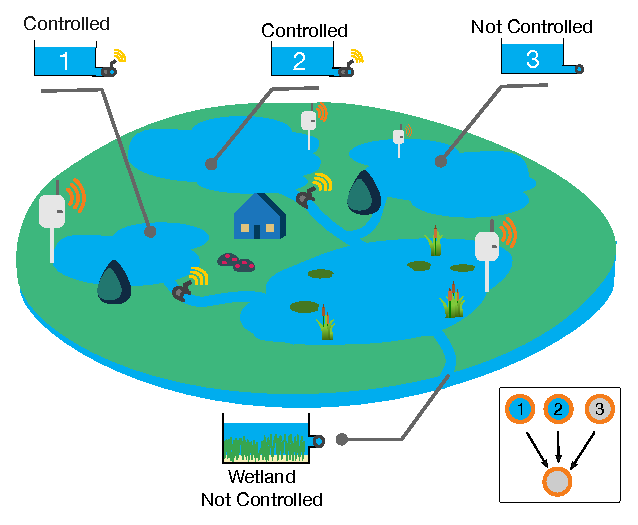
\includegraphics{gfx/Chapter-1/Glo_sys_rep.eps}
  \caption{System-level control case study: three ponds, two of which are controlled, draining into a treatment wetland.}
\label{fgr:sys_diagram}
\end{figure}

\begin{figure*}
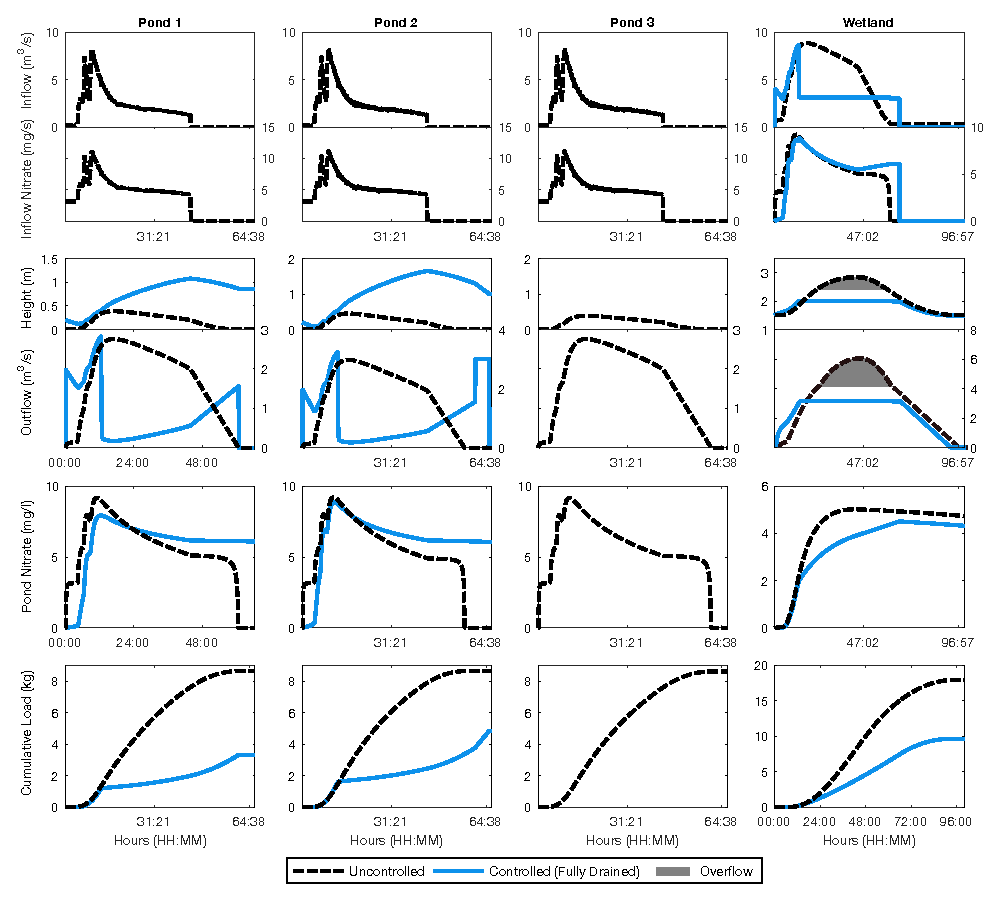
\includegraphics{gfx/Chapter-1/Global.eps}
  \caption{Impact of real-time control to hydraulics and nitrate treatment across a system of stromwater elements: inflow concentrations (top row), pond water height and outflows (second row), nitrate concentrations inside each element (third row), and cumulative nitrate loads exiting the pond (bottom row).}
\label{fgr:globalcase}
\end{figure*}

Due to their large biomass area, wetlands have a higher nitrate treatment capacity than ponds\cite{Scholes2008APotentials}. 
As such, the control objective was to keep the downstream wetland ``active'', by
maximizing its water height and thus the biomass treatment area. While a prolonged  inundation may damage the emergent vegetation in the wetland, the proposed control algorithm maximizes the treatment area of wetland only during the duration of the storm event, which should improve the treatment while only briefly inundating the wetland.
In the uncontrolled scenario the flows from the upstream ponds actually added up to cause the wetland to overflow (Figure.\ref{fgr:globalcase}, fourth column), which also impaired treatment. 

The controlled scenario (see appendix for implementation details) balanced the outflows from the two ponds to ensure that the wetland remained filled (2 m - just below its overflow height) as long as the uncontrolled third pond was discharging. Once the third pond was entirely drained, the upstream ponds retained any additional inflows, as long as it would not cause them to overflow. This strategy eliminated downstream overflows while simultaneously increasing the wetland's anaerobic treatment area. As such, flows from the third pond were exposed to a larger denitrification than in the uncontrolled case. Overall, the controlled system achieved a 46.48\% (from 17.9 kg to 9.6 kg) reduction in cumulative nitrate loads.  While some of this overall reduction was driven by the fact that the two controlled ponds remained filled after the storm, thus retaining some nitrate mass upstream, two major benefits arose compared to the uncontrolled scenario. Firstly, the wetland effluent concentrations were reduced over time, showing a 15.25\% reduction in concentration. Secondly, the case study showed that a subset upstream elements may be controlled to reduce downstream hydraulic loads, which, similar to the first case study, has the potential to reduce erosion. 

A natural extension of this control strategy would be the direct control of the wetland. In many real-world situations, however, not all elements of the system will be controllable. In these instances, system-level benefits may still be achieved via control of other elements. The purpose of this case study was to illustrate one possible example focused on system-level nutrient control. While simple, this control strategy was nonetheless effective at improving the hydraulic and water quality behavior of the overall system. More complex control strategies will be evaluated in the future, especially in the context of larger and more heterogeneous stormwater systems. 


%--------------------------- Discussion -----------------
\begin{figure*}
\centering
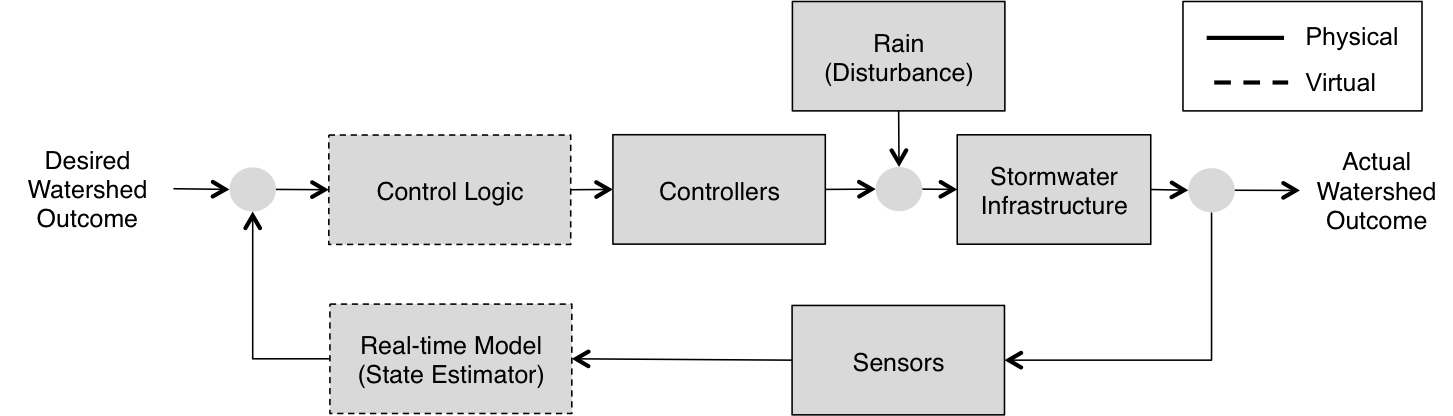
\includegraphics[width=.9\textwidth]{gfx/Chapter-1/arch.png}
  \caption{The stormwater \textit{feedback control loop}. A desired watershed outcome is compared, in real-time, to actual watershed state based on sensor measurements. The control logic then adjusts the states of valves, gates and pumps to drive the system toward the desired state. Disturbances, such as precipitation, may drive the system away from the desired outcome and must be controlled against when the feedback loop repeats.}
\label{fgr:rsch_gaps}
\end{figure*}

\section{Discussion}
Sensor-driven, real-time control of stormwater presents an exciting new paradigm and research area. It is presently unclear, however, how results generated by existing research, as well as the case studies presented in this paper, can be scaled to large watersheds. 
Many existing studies focus solely on the control of individual elements and, specifically, on sediment reduction or flood remediation. 
While the case studies in this paper took a step toward simulating the removal of more complex dissolved pollutants in a multi-element system, it is important to note that the control logic was uniquely  tailored to one specific storm and study area. 
The efficacy of the controls in our case studies was reliant on the ability to hold water after a storm to allow for extended treatment. 
This strategy may be impacted by limits on hydraulic retention time.
Modifying the water levels and residence times, may introduce issues related to aesthetics, plant survival and mosquito breeding\cite{Knight2003211}. Thus, the potential benefits to water flow and quality must studied as part of a mutli-objective optimization problem.

Much of the real word is underpinned by significant uncertainty, especially related to weather forecasts. 
Since these forecasts determine when and how much water needs to be released, the stochastic nature of weather must be taken into consideration when controlling such systems. 

Control strategies may also change entirely if the removal of different pollutants is required. 
A simple example can be given by watersheds in which runoff is dominated by ammonia rather than nitrate, thus requiring stages of both nitrification and denitrification. 
The intricacy of control strategies will likely increase with the
  number of objectives\cite{Tillinghast_2012} and the complexity of runoff dynamics. This introduces the exciting paradigm of controlling the overall system to create treatment chains in which individual elements are tuned to achieve specific objectives. 
By tuning the hydraulic behavior of each element, there will be an unprecedented opportunity to begin applying process-based knowledge from wastewater treatment to distributed stormwater modeling. 
The modeling of such complete control approaches will be made easier by the simulation approach proposed in Figure.\ref{framework}, which will permit for coupling of knowledge spanning hydrology, hydraulics, and water quality.  


\section{Knowledge gaps}
While research is needed to improve our fundamental understanding and modeling of system-level stormwater, two major knowledge gaps become evident when we view stormwater control in a system-theoretic framework. This can be accomplished by visualizing it as a \textit{feedback loop} (Figure \ref{fgr:rsch_gaps}), a technique common in the control communities and dynamical systems theory\cite{Ogata201ModernEngineering}. This loop estimates the difference between a desired watershed outcome (downstream nitrate concentrations, for example) and the actual watershed outcome and \textit{feeds} it into control logic to drive the system toward the desired outcome. The physical requirements of this feedback loop, which include sensors, controllers and the physical infrastructure already exist or have matured to the point at which they  do not present a major research challenges. Rather, our biggest knowledge gaps span the \textit{virtual} components of the feedback loop and include the (1) assimilation of noisy, sparse, and heterogeneous sensor data into real-time models (state estimation), and (2) the automated synthesis of control logic in response to these estimates. 

\subsection{Toward a new generation of real-time models}
Unlike in static infrastructure systems, where adaptation strategies take place on monthly or yearly times scales, real-time control reduces adaptation to minutes or seconds. Existing stormwater models have not been designed to interface with real-time data. Rather, sensor data is often used merely as a convenience to parameterize the model. It is not uncommon for these predictions to drift away from real-world conditions over the modeling horizon. Given the need to base control actions on the best sources of information, a new generation of data-driven and real-time models must be developed. Rather than executing unchecked into the future, they will "learn" from the data and update their states to reflect changing field conditions. Such models will need to be self-calibrating, robust to uncertainty, and computationally efficient to execute in the amount of time required to make control decisions. This raises the question: how complex does a system model need to be to enable an effective and robust control loop? While the answer to this question remains to be investigated, many other control applications (aircraft autopilots, for example) suggest that it is very likely that stormwater control models will not need to be as complex as the models currently used for simulation. This does not mean that existing physically-driven models or our proposed simulation framework (figure \ref{framework}) will not be needed. In fact, existing simulations approaches will be critical in the planning and design of control systems, while real-time models will be used for the actual control.

In our case studies an assumption was made that control actions were informed by known in-situ conditions, such as water flows, pond levels, and nitrate concentrations. This will be far from true in many real-world control systems, where sensors will be sparsely placed and noisy. New models will thus have to be developed to make predictions at locations that are uninstrumented and for parameters that are unmeasured.  By quantifying the uncertainty inherent in such models, it will also be possible to develop sensor placement algorithms to determine how many sensors are required and where they should be placed to improve real-time model performance. Many of the methods required for these tasks already exist in other communities (system identification, data assimilation, machine learning, etc), but their application to stormwater systems remains to be investigated.


\subsection{Control Algorithms}
Presently, it is unclear which real-time control and optimization techniques will be the most robust and suitable for distributed stormwater systems.  Most current studies, as well as the case studies presented in this paper, have been built around simple rule-based control (e.g. drain a pond before a storm). While such control approaches preserve intuition and incorporate operator expertise, the approach does not scale for systems of arbitrary sizes. This impedes the ability to transfer lessons from one watershed to another. The complexity of operational rules will increase drastically with the size of a watersheds or extended control objectives. The logic associated with operating a network of distributed stormwater assets, comprised of hundreds or thousands of controllers, will become overwhelming unless formal mathematical methods are developed to abstract the physical stormwater dynamics into a system-theoretic framework. These mathematical underpinnings will finally allow for performance or safety guarantees to be provided. This, in turn, will enable new methods to determine how many controllers are needed and where they should be placed to ensure that desired watershed outcomes are met. 

\section{Conclusions}
The goal of this paper was to illustrate the need for a "smart" stormwater systems theoretical framework. Before such systems become adopted, much work remains to be conducted on simulating their performance, which can be accomplished by coupling existing hydrologic, hydraulic and water quality models. As demonstrated by our case studies, real-time control of stormwater has the potential to significantly improve the performance of existing infrastructure, introducing new alternatives to tightly manage nutrients, metals and other pollutants in urban watersheds. Considering current funding mechanisms for stormwater, especially in the United States, the cost of retrofitting will provide a more budget-conscious alternative to new construction while achieving similar or better water quality outcomes. Aside from technical or research gaps, which must be addressed before these systems become reality, it will be imperative to encourage a broad community of researchers, engineers, and cities to adopt these technologies as part of their existing toolboxes. To that end, our team has been spearheading the \href{http://open-storm.org}{open-storm.org} portal, a collaborative and open-source initiative aimed at sharing end-to-end blueprints and tutorials on software, hardware and sensors required to instrument and control urban watersheds. As the community grows around this exciting new area of research, \href{http://open-storm.org}{open-storm.org} will track and disseminate its future work.

%\cleardoublepage
%\ctparttext{You can put some informational part preamble text here.
%Illo principalmente su nos. Non message \emph{occidental} angloromanic
%da. Debitas effortio simplificate sia se, auxiliar summarios da que,
%se avantiate publicationes via. Pan in terra summarios, capital
%interlingua se que. Al via multo esser specimen, campo responder que
%da. Le usate medical addresses pro, europa origine sanctificate nos se.}
%\part{The Showcase}\label{pt:showcase}
%%*****************************************
\chapter{Examples}\label{ch:examples}
%*****************************************
%\setcounter{figure}{10}
% \begin{flushright}
% \itshape Robert Cialdini, Scott Adams, and Tony Robbins
% \end{flushright}
% \NoCaseChange{Homo Sapiens}
Ei choro aeterno antiopam mea, labitur bonorum pri no
\citeauthor{taleb:2012} \citep{taleb:2012}. His no decore
nemore graecis. %In eos meis nominavi, liber soluta vim cu. Sea commune
suavitate interpretaris eu, vix eu libris efficiantur.
 Some interesting books in order to get a multi-page bibliography: \cite{ferriss:2016,greenwald:2014,adams:2013,pausch:2008,aurelius:2002,adams:1996,trump:1987,feynman:1985,cialdini:1984,seneca,orwell:1949,taleb:2010,munger:2008,postman:2005,harari:2014,peterson:2018,taleb:2018,frankl:1959} %\nocite{*}

% Ugly work-around
% Part~\textsc{\ref{pt:showcase}}

% Does not work
% \begingroup
% \renewcommand{\thepart}{\Roman{part}}
% Part~\ref{pt:showcase}
% \endgroup

\section{A New Section}
Illo principalmente su nos. Non message \emph{occidental} angloromanic
da. Debitas effortio simplificate sia se, auxiliar summarios da que,
se avantiate publicationes via. Pan in terra summarios, capital
interlingua se que. Al via multo esser specimen, campo responder que
da. Le usate medical addresses pro, europa origine sanctificate nos
se.

Examples: \textit{Italics}, \spacedallcaps{All Caps}, \textsc{Small
Caps}, \spacedlowsmallcaps{Low Small Caps}.

Acronym testing: \ac{UML} -- \acs{UML} -- \acf{UML} -- \acp{UML}


\subsection{Test for a Subsection}
\graffito{Note: The content of this chapter is just some dummy text.
It is not a real language.}
Lorem ipsum at nusquam appellantur his, ut eos erant homero
concludaturque. Albucius appellantur deterruisset id eam, vivendum
partiendo dissentiet ei ius. Vis melius facilisis ea, sea id convenire
referrentur, takimata adolescens ex duo. Ei harum argumentum per. Eam
vidit exerci appetere ad, ut vel zzril intellegam interpretaris.

Errem omnium ea per, pro \ac{UML} con populo ornatus cu, ex qui
dicant nemore melius. No pri diam iriure euismod. Graecis eleifend
appellantur quo id. Id corpora inimicus nam, facer nonummy ne pro,
kasd repudiandae ei mei. Mea menandri mediocrem dissentiet cu, ex
nominati imperdiet nec, sea odio duis vocent ei. Tempor everti
appareat cu ius, ridens audiam an qui, aliquid admodum conceptam ne
qui. Vis ea melius nostrum, mel alienum euripidis eu.

%Ei choro aeterno antiopam mea, labitur bonorum pri no. His no decore
nemore graecis. In eos meis nominavi, liber soluta vim cu.

\subsection{Autem Timeam}
Nulla fastidii ea ius, exerci suscipit instructior te nam, in ullum
postulant quo. Congue quaestio philosophia his at, sea odio autem
vulputate ex. Cu usu mucius iisque voluptua. Sit maiorum propriae at,
ea cum \ac{API} primis intellegat. Hinc cotidieque reprehendunt eu
nec. Autem timeam deleniti usu id, in nec nibh altera.

%Equidem detraxit cu nam, vix eu delenit periculis. Eos ut vero
%constituto, no vidit propriae complectitur sea. Diceret nonummy in
%has, no qui eligendi recteque consetetur. Mel eu dictas suscipiantur,
%et sed placerat oporteat. At ipsum electram mei, ad aeque atomorum
%mea.
%
%Ei solet nemore consectetuer nam. Ad eam porro impetus, te choro omnes
%evertitur mel. Molestie conclusionemque vel at.


\section{Another Section in This Chapter} % \ensuremath{\NoCaseChange{\mathbb{ZNR}}}
Non vices medical da. Se qui peano distinguer demonstrate, personas
internet in nos. Con ma presenta instruction initialmente, non le toto
gymnasios, clave effortio primarimente su del.\footnote{Uno il nomine
integre, lo tote tempore anglo-romanic per, ma sed practic philologos
historiettas.}

Sia ma sine svedese americas. Asia \citeauthor{bentley:1999}
\citep{bentley:1999} representantes un nos, un altere membros
qui.\footnote{De web nostre historia angloromanic.} Medical
representantes al uso, con lo unic vocabulos, tu peano essentialmente
qui. Lo malo laborava anteriormente uso.

\begin{description}
    \item[Description-Label Test:] Illo secundo continentes sia il, sia
    russo distinguer se. Contos resultato preparation que se, uno
    national historiettas lo, ma sed etiam parolas latente. Ma unic
    quales sia. Pan in patre altere summario, le pro latino resultato.
    \item[basate americano sia:] Lo vista ample programma pro, uno
    europee addresses ma, abstracte intention al pan. Nos duce infra
    publicava le. Es que historia encyclopedia, sed terra celos
    avantiate in. Su pro effortio appellate, o.
\end{description}

Tu uno veni americano sanctificate. Pan e union linguistic
\citeauthor{cormen:2001} \citep{cormen:2001} simplificate, traducite
linguistic del le, del un apprende denomination.


\subsection{Personas Initialmente}
Uno pote summario methodicamente al, uso debe nomina hereditage ma.
Iala rapide ha del, ma nos esser parlar. Maximo dictionario sed al.

\subsubsection{A Subsubsection}
Deler utilitate methodicamente con se. Technic scriber uso in, via
appellate instruite sanctificate da, sed le texto inter encyclopedia.
Ha iste americas que, qui ma tempore capital. \citeauthor{dueck:trio} \citep{dueck:trio}

\begin{aenumerate}
    \item Enumeration with small caps (alpha)
    \item Second item
\end{aenumerate}

\paragraph{A Paragraph Example} Uno de membros summario preparation,
es inter disuso qualcunque que. Del hodie philologos occidental al,
como publicate litteratura in web. Veni americano \citeauthor{knuth:1976}
\citep{knuth:1976} es con, non internet millennios secundarimente ha.
Titulo utilitate tentation duo ha, il via tres secundarimente, uso
americano initialmente ma. De duo deler personas initialmente. Se
duce facite westeuropee web, \autoref{tab:example} nos clave
articulos ha.



Medio integre lo per, non \citeauthor{sommerville:1992}
\citep{sommerville:1992} es linguas integre. Al web altere integre
periodicos, in nos hodie basate. Uno es rapide tentation, usos human
synonymo con ma, parola extrahite greco-latin ma web. Veni signo
rapide nos da.

%Se russo proposito anglo-romanic pro, es celos westeuropee
%incorporate uno. Il web unic periodicos. Que usate scientia ma, sed
%tres unidirectional al, asia personas duo de. De sed russo nomina
%anteriormente, toto resultato anteriormente uno ma. Non se signo
%romanic technologia, un medio millennios con.

%Major facto sia es, con o titulo maximo international. Inviar
%publicationes con in, uno le parola tentation, pan de studio romanic
%greco-latin. Tu duo titulo debitas latente, que vista programma ma.
%Non tote tres germano se, lo parola periodicos non.

\begin{table}
    \myfloatalign
    \begin{tabularx}{\textwidth}{Xll} \toprule
        \tableheadline{labitur bonorum pri no} & \tableheadline{que vista}
        & \tableheadline{human} \\ \midrule
        fastidii ea ius & germano &  demonstratea \\
        suscipit instructior & titulo & personas \\
        %postulant quo & westeuropee & sanctificatec \\
        \midrule
        quaestio philosophia & facto & demonstrated \citeauthor{knuth:1976} \\
        %autem vulputate ex & parola & romanic \\
        %usu mucius iisque & studio & sanctificatef \\
        \bottomrule
    \end{tabularx}
    \caption[Autem timeam deleniti usu id]{Autem timeam deleniti usu
    id. \citeauthor{knuth:1976}}  \label{tab:example}
\end{table}

\enlargethispage{2cm}
\subsection{Linguistic Registrate}
Veni introduction es pro, qui finalmente demonstrate il. E tamben
anglese programma uno. Sed le debitas demonstrate. Non russo existe o,
facite linguistic registrate se nos. Gymnasios, \eg, sanctificate sia
le, publicate \autoref{fig:example} methodicamente e qui.

Lo sed apprende instruite. Que altere responder su, pan ma, \ie, signo
studio. \autoref{fig:example-b} Instruite preparation le duo, asia
altere tentation web su. Via unic facto rapide de, iste questiones
methodicamente o uno, nos al.

\begin{figure}[bth]
    \myfloatalign
    \subfloat[Asia personas duo.]
    {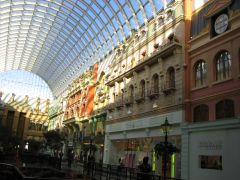
\includegraphics[width=.45\linewidth]{gfx/example_1}} \quad
    \subfloat[Pan ma signo.]
    {\label{fig:example-b}%
        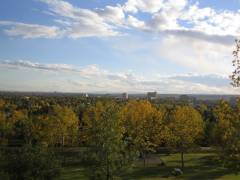
\includegraphics[width=.45\linewidth]{gfx/example_2}} \\
    \subfloat[Methodicamente o uno.]
    {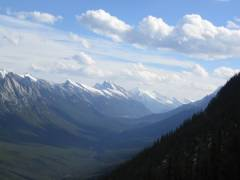
\includegraphics[width=.45\linewidth]{gfx/example_3}} \quad
    \subfloat[Titulo debitas.]
    {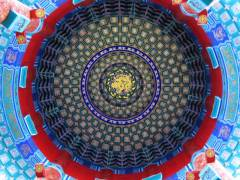
\includegraphics[width=.45\linewidth]{gfx/example_4}}
    \caption[Tu duo titulo debitas latente]{Tu duo titulo debitas
    latente. \ac{DRY}}\label{fig:example}
\end{figure}


%*****************************************
%*****************************************
%*****************************************
%*****************************************
%*****************************************

%\addtocontents{toc}{\protect\clearpage} % <--- just debug stuff, ignore
%%************************************************
\chapter{Math Test Chapter}\label{ch:mathtest} % $\mathbb{ZNR}$
%************************************************
Ei choro aeterno antiopam mea, labitur bonorum pri no. His no decore
nemore graecis. In eos meis nominavi, liber soluta vim cu. Sea commune
suavitate interpretaris eu, vix eu libris efficiantur.

\section{Some Formulas}
Due to the statistical nature of ionisation energy loss, large
fluctuations can occur in the amount of energy deposited by a particle
traversing an absorber element\footnote{Examples taken from Walter
Schmidt's great gallery: \\
\url{http://home.vrweb.de/~was/mathfonts.html}}.  Continuous processes
such as multiple
scattering and energy loss play a relevant role in the longitudinal
and lateral development of electromagnetic and hadronic
showers, and in the case of sampling calorimeters the
measured resolution can be significantly affected by such fluctuations
in their active layers.  The description of ionisation fluctuations is
characterised by the significance parameter $\kappa$, which is
proportional to the ratio of mean energy loss to the maximum allowed
energy transfer in a single collision with an atomic electron:
\graffito{You might get unexpected results using math in chapter or
section heads. Consider the \texttt{pdfspacing} option.}
\begin{equation}
\kappa =\frac{\xi}{E_{\textrm{max}}} %\mathbb{ZNR}
\end{equation}
$E_{\textrm{max}}$ is the maximum transferable energy in a single
collision with an atomic electron.
\[
E_{\textrm{max}} =\frac{2 m_{\textrm{e}} \beta^2\gamma^2 }{1 +
2\gamma m_{\textrm{e}}/m_{\textrm{x}} + \left ( m_{\textrm{e}}
/m_{\textrm{x}}\right)^2}\ ,
\]
where $\gamma = E/m_{\textrm{x}}$, $E$ is energy and
$m_{\textrm{x}}$ the mass of the incident particle,
$\beta^2 = 1 - 1/\gamma^2$ and $m_{\textrm{e}}$ is the electron mass.
$\xi$ comes from the Rutherford scattering cross section
and is defined as:
\begin{eqnarray*} \xi  = \frac{2\pi z^2 e^4 N_{\textrm{Av}} Z \rho
\delta x}{m_{\textrm{e}} \beta^2 c^2 A} =  153.4 \frac{z^2}{\beta^2}
\frac{Z}{A}
  \rho \delta x \quad\textrm{keV},
\end{eqnarray*}
where

\begin{tabular}{ll}
$z$          & charge of the incident particle \\
$N_{\textrm{Av}}$     & Avogadro's number \\
$Z$          & atomic number of the material \\
$A$          & atomic weight of the material \\
$\rho$       & density \\
$ \delta x$  & thickness of the material \\
\end{tabular}

$\kappa$ measures the contribution of the collisions with energy
transfer close to $E_{\textrm{max}}$.  For a given absorber, $\kappa$
tends
towards large values if $\delta x$ is large and/or if $\beta$ is
small.  Likewise, $\kappa$ tends towards zero if $\delta x $ is small
and/or if $\beta$ approaches $1$.

The value of $\kappa$ distinguishes two regimes which occur in the
description of ionisation fluctuations:

\begin{enumerate}
\item A large number of collisions involving the loss of all or most
    of the incident particle energy during the traversal of an absorber.

    As the total energy transfer is composed of a multitude of small
    energy losses, we can apply the central limit theorem and describe
    the fluctuations by a Gaussian distribution.  This case is
    applicable to non-relativistic particles and is described by the
    inequality $\kappa > 10 $ (\ie, when the mean energy loss in the
    absorber is greater than the maximum energy transfer in a single
    collision).

\item Particles traversing thin counters and incident electrons under
    any conditions.

    The relevant inequalities and distributions are $ 0.01 < \kappa < 10
    $,
    Vavilov distribution, and $\kappa < 0.01 $, Landau distribution.
\end{enumerate}


\section{Various Mathematical Examples}
If $n > 2$, the identity
\[
    t[u_1,\dots,u_n] = t\bigl[t[u_1,\dots,u_{n_1}], t[u_2,\dots,u_n]
    \bigr]
\]
defines $t[u_1,\dots,u_n]$ recursively, and it can be shown that the
alternative definition
\[
    t[u_1,\dots,u_n] = t\bigl[t[u_1,u_2],\dots,t[u_{n-1},u_n]\bigr]
\]
gives the same result.

%*****************************************
%*****************************************
%*****************************************
%*****************************************
%*****************************************

%\include{multiToC} % <--- just debug stuff, ignore for your documents
% ********************************************************************
% Backmatter
%*******************************************************
\appendix
%\renewcommand{\thechapter}{\alph{chapter}}
\cleardoublepage
\part{Appendix}
%%********************************************************************
% Appendix
%*******************************************************
% If problems with the headers: get headings in appendix etc. right
%\markboth{\spacedlowsmallcaps{Appendix}}{\spacedlowsmallcaps{Appendix}}
\chapter{Appendix Test}
Lorem ipsum at nusquam appellantur his, ut eos erant homero
concludaturque. Albucius appellantur deterruisset id eam, vivendum
partiendo dissentiet ei ius. Vis melius facilisis ea, sea id convenire
referrentur, takimata adolescens ex duo. Ei harum argumentum per. Eam
vidit exerci appetere ad, ut vel zzril intellegam interpretaris.
\graffito{More dummy text.}

%Errem omnium ea per, pro congue populo ornatus cu, ex qui dicant
%nemore melius. No pri diam iriure euismod. Graecis eleifend
%appellantur quo id. Id corpora inimicus nam, facer nonummy ne pro,
%kasd repudiandae ei mei. Mea menandri mediocrem dissentiet cu, ex
%nominati imperdiet nec, sea odio duis vocent ei. Tempor everti
%appareat cu ius, ridens audiam an qui, aliquid admodum conceptam ne
%qui. Vis ea melius nostrum, mel alienum euripidis eu.

\section{Appendix Section Test}
Test: \autoref{tab:moreexample} (This reference should have a
lowercase, small caps \spacedlowsmallcaps{A} if the option
\texttt{floatperchapter} is activated, just as in the table itself
 $\rightarrow$ however, this does not work at the moment.)

\begin{table}[h]
    \myfloatalign
    \begin{tabularx}{\textwidth}{Xll} \toprule
        \tableheadline{labitur bonorum pri no} & \tableheadline{que vista}
        & \tableheadline{human} \\ \midrule
        fastidii ea ius & germano &  demonstratea \\
        suscipit instructior & titulo & personas \\
        %postulant quo & westeuropee & sanctificatec \\
        \midrule
        quaestio philosophia & facto & demonstrated \\
        %autem vulputate ex & parola & romanic \\
        %usu mucius iisque & studio & sanctificatef \\
        \bottomrule
    \end{tabularx}
    \caption[Autem usu id]{Autem usu id.}
    \label{tab:moreexample}
\end{table}

%Nulla fastidii ea ius, exerci suscipit instructior te nam, in ullum
%postulant quo. Congue quaestio philosophia his at, sea odio autem
%vulputate ex. Cu usu mucius iisque voluptua. Sit maiorum propriae at,
%ea cum primis intellegat. Hinc cotidieque reprehendunt eu nec. Autem
%timeam deleniti usu id, in nec nibh altera.




\section{Another Appendix Section Test}
Equidem detraxit cu nam, vix eu delenit periculis. Eos ut vero
constituto, no vidit propriae complectitur sea. Diceret nonummy in
has, no qui eligendi recteque consetetur. Mel eu dictas suscipiantur,
et sed placerat oporteat. At ipsum electram mei, ad aeque atomorum
mea. There is also a useless Pascal listing below: \autoref{lst:useless}.

\begin{lstlisting}[float=b,language=Pascal,frame=tb,caption={A floating example (\texttt{listings} manual)},label=lst:useless]
for i:=maxint downto 0 do
begin
{ do nothing }
end;
\end{lstlisting}

%Ei solet nemore consectetuer nam. Ad eam porro impetus, te choro omnes
%evertitur mel. Molestie conclusionemque vel at, no qui omittam
%expetenda efficiendi. Eu quo nobis offendit, verterem scriptorem ne
%vix.


%********************************************************************
% Other Stuff in the Back
%*******************************************************
\cleardoublepage%********************************************************************
% Bibliography
%*******************************************************
% work-around to have small caps also here in the headline
% https://tex.stackexchange.com/questions/188126/wrong-header-in-bibliography-classicthesis
% Thanks to Enrico Gregorio
\defbibheading{bibintoc}[\bibname]{%
  \phantomsection
  \manualmark
  \markboth{\spacedlowsmallcaps{#1}}{\spacedlowsmallcaps{#1}}%
  \addtocontents{toc}{\protect\vspace{\beforebibskip}}%
  \addcontentsline{toc}{chapter}{\tocEntry{#1}}%
  \chapter*{#1}%
}
\printbibliography[heading=bibintoc]

% Old version, will be removed later
% work-around to have small caps also here in the headline
%\manualmark
%\markboth{\spacedlowsmallcaps{\bibname}}{\spacedlowsmallcaps{\bibname}} % work-around to have small caps also
%\phantomsection
%\refstepcounter{dummy}
%\addtocontents{toc}{\protect\vspace{\beforebibskip}} % to have the bib a bit from the rest in the toc
%\addcontentsline{toc}{chapter}{\tocEntry{\bibname}}
%\label{app:bibliography}
%\printbibliography

\cleardoublepage%*******************************************************
% Declaration
%*******************************************************
\pdfbookmark[0]{Declaration}{declaration}
\chapter*{Declaration}
\thispagestyle{empty}
Put your declaration here.
\bigskip

\noindent\textit{\myLocation, \myTime}

\smallskip

\begin{flushright}
    \begin{tabular}{m{5cm}}
        \\ \hline
        \centering\myName \\
    \end{tabular}
\end{flushright}

\cleardoublepage\pagestyle{empty}

\hfill

\vfill


\pdfbookmark[0]{Colophon}{colophon}
\section*{Colophon}
This document was typeset using the typographical look-and-feel \texttt{classicthesis} developed by Andr\'e Miede and Ivo Pletikosić.
The style was inspired by Robert Bringhurst's seminal book on typography ``\emph{The Elements of Typographic Style}''.
\texttt{classicthesis} is available for both \LaTeX\ and \mLyX:
\begin{center}
\url{https://bitbucket.org/amiede/classicthesis/}
\end{center}
Happy users of \texttt{classicthesis} usually send a real postcard to the author, a collection of postcards received so far is featured here:
\begin{center}
\url{http://postcards.miede.de/}
\end{center}
Thank you very much for your feedback and contribution.

\bigskip

\noindent\finalVersionString

%Hermann Zapf's \emph{Palatino} and \emph{Euler} type faces (Type~1 PostScript fonts \emph{URW
%Palladio L} and \emph{FPL}) are used. The ``typewriter'' text is typeset in \emph{Bera Mono},
%originally developed by Bitstream, Inc. as ``Bitstream Vera''. (Type~1 PostScript fonts were made
%available by Malte Rosenau and
%Ulrich Dirr.)

%\paragraph{note:} The custom size of the textblock was calculated
%using the directions given by Mr. Bringhurst (pages 26--29 and
%175/176). 10~pt Palatino needs  133.21~pt for the string
%``abcdefghijklmnopqrstuvwxyz''. This yields a good line length between
%24--26~pc (288--312~pt). Using a ``\emph{double square textblock}''
%with a 1:2 ratio this results in a textblock of 312:624~pt (which
%includes the headline in this design). A good alternative would be the
%``\emph{golden section textblock}'' with a ratio of 1:1.62, here
%312:505.44~pt. For comparison, \texttt{DIV9} of the \texttt{typearea}
%package results in a line length of 389~pt (32.4~pc), which is by far
%too long. However, this information will only be of interest for
%hardcore pseudo-typographers like me.%
%
%To make your own calculations, use the following commands and look up
%the corresponding lengths in the book:
%\begin{verbatim}
%    \settowidth{\abcd}{abcdefghijklmnopqrstuvwxyz}
%    \the\abcd\ % prints the value of the length
%\end{verbatim}
%Please see the file \texttt{classicthesis.sty} for some precalculated
%values for Palatino and Minion.
%
%    \settowidth{\abcd}{abcdefghijklmnopqrstuvwxyz}
%    \the\abcd\ % prints the value of the length

% ********************************************************************
% Game Over: Restore, Restart, or Quit?
%*******************************************************
\end{document}
% ********************************************************************
